% !TEX program = arara
% !TEX options = -v %DOC%

% arara: xelatex
% arara: makeglossaries
% arara: xelatex

\documentclass[openany, twoside, b5paper]{memoir}

\usepackage[b5paper]{geometry}
\brokenpenalty=1000
\clubpenalty=1000
\widowpenalty=1000

\usepackage{libertine}

\usepackage{microtype} % Improves spacing


% Layout for title page, cf. titlepages package
\newlength\drop
\makeatletter
\newcommand*{\titleS}{\begingroup% Scripts, T&H p 151
\drop = 0.1\textheight
\centering
\vspace*{\drop}
{\large Koolder mal Erlehirni}\\[2\baselineskip]
{\Huge Andro Grammar Handbook}\\[\baselineskip]
\vfill
%{\large\itshape Benung.\ The Ayeri Language Resource}\\
%\rule{0.5\textwidth}{0.4pt}\smallskip\\
{Koolder mal Erlehirni\\ Lublin, Poland · 2021}\par
\vspace*{\drop}
\endgroup}
\makeatother

% Layout for running page titles
\nouppercaseheads
\copypagestyle{sfheaders}{headings}
\makeevenhead{sfheaders}{\sffamily{\bfseries\thepage}\quad{\itshape\leftmark}}{}{}
\makeoddhead{sfheaders}{}{}{\sffamily{\itshape\rightmark}\quad\bfseries\thepage}
% \makeheadrule{headings}{\textwidth}{0.3pt}
\pagestyle{sfheaders}

% Layout for Notes pages
\copypagestyle{notes}{headings}
\makeevenhead{notes}{}{\sffamily{\bfseries Notes}}{}
\makeoddhead{notes}{}{\sffamily{\bfseries Notes}}{}

% Layout for chapter headers
\chapterstyle{southall}
\renewcommand*{\chaptitlefont}{\huge\sffamily\raggedright}

% Sectioning depth
\setcounter{secnumdepth}{2} % doesn't work for some reason
\setsecnumdepth{subsection}
\settocdepth{subsection}

% Space requirements
% \usepackage{needspace}

% Calculation stuff
% \usepackage{calc}

% Load fonts for XeTeX, including support for Unicode etc.
% Mathspec makes it possible to redefine *all* the fonts used for math stuff,
% however, it contains a stupid bug in dependency checking, see
% <http://tex.stackexchange.com/a/85700>.
% \usepackage{mathspec}
% \makeatletter
% % undo the wrong changes made by mathspec
% \let\RequirePackage\original@RequirePackage
% \let\usepackage\RequirePackage

\usepackage{xunicode}
\usepackage{xltxtra}

% Handle language and quotation marks
\usepackage{polyglossia}
\setdefaultlanguage[variant=american]{english}
\usepackage[
	style=american,
	english=american,
	autopunct,
]{csquotes} % Put quotations in \enquote{} or \textquote{}!
\SetBlockEnvironment{quote}
\renewcommand*{\mkccitation}[1]{ (#1)}

% Date and time
% \usepackage[useregional]{datetime2}

% Extended formatting of lists
% \usepackage{enumitem}
% \newlist{glossdefs}{itemize}{1}
% \setlist[glossdefs]{nosep, leftmargin=4.5em, labelwidth=4em, align=left}
% \setlist[itemize]{noitemsep}
% \setlist[description]{font=\sffamily\bfseries}

% Make multiple columns available in single-column document
% \usepackage{multicol}

% Relative font sizes
% \usepackage{relsize}

% Nicer footnotes
\usepackage[bottom,hang,norule]{footmisc}
\setlength{\footnotesep}{0.75\baselineskip}

% Things for tables; needs to be loaded *before* hyperref if footnotes in
% tables are supposed to work (bug in tabu where they still don't?)
% \usepackage{longtable}
% \usepackage{tabu}
% \usepackage{booktabs}
% \usepackage{bigstrut}
% \usepackage{array}
% \usepackage{adjustbox}
% \usepackage{makecell}
% \AtBeginEnvironment{tabu}{\smaller}
% \usepackage{rotating}
% \usepackage{multirow}

% \tabulinesep = .5\itemsep

% \newenvironment{morphlex}{%
% 	\tabulinesep = 0pt%
% }{%
% \ignorespacesafterend%
% }

% Dealing with page-size tables in landscape format
% http://tex.stackexchange.com/a/19021, and hat tip to Git user Zoqaeski:
% \usepackage{pdflscape} % alternative to rotating; rotates pages on screen
% \usepackage{afterpage} % put things after the page they're defined on

% Appendices
\usepackage{appendix}

% Custom column types
\newcolumntype{B}{>{\bfseries}X}
\newcolumntype{I}{>{\itshape}X}
\newcolumntype{H}{>{\bfseries\footnotesize}X}
\newcolumntype{S}{>{\footnotesize}X}
\newcolumntype{C}{>{\scshape}X}

% Table header font
% \newcommand{\tableheaderfont}{\rowfont{\upshape\bfseries}}
% \newcommand{\tablesubheaderfont}{\rowfont{\upshape\bfseries\footnotesize}}

% Clickable links in footnotes, TOC, etc.
% \usepackage[
% 	xetex,
% 	pdfusetitle,
% 	bookmarks,
% 	linktoc=section,
% 	colorlinks=false,
% 	hidelinks,
% ]{hyperref}

% Write "section" instead of "subsection", "subsubsection" etc.
\let\subsectionautorefname\sectionautorefname
\let\subsubsectionautorefname\sectionautorefname

% Formatting of URLs
% \DeclareFieldFormat{url}{\href{#1}{\itshape #1}}
% \def\UrlNoBreaks{\do\(\do\[\do\{\do\<\do\:}
% \urlstyle{same}

% Ability to include graphics and dealing with footnotes in descriptions
\usepackage{graphicx}
\usepackage[
	font={small,sf},
	labelfont={small,sf},
	format=plain,
	skip=.25\baselineskip
]{caption}
\graphicspath{ {../images/} }

% Increase rubber between a float and text. Otherwise, we may get up to a
% line's worth of whitespace between paragraphs when a float is at the top.
% (https://tex.stackexchange.com/a/26522)
% \setlength{\textfloatsep}{20pt plus 8pt minus 4pt}

% Throughout the book, examples are wrapped in floats to dynamically position 
% them. By default, LaTeX tries to put floats at the top of pages, disrupting 
% the reading flow. For examples especially, thus, we want them to be placed 
% 'here', if possible, or at the top of the next page (cf. 'memoir' package 
% manual, p. 177f.)
\setfloatlocations{figure}{htbp}

% \usepackage{subcaption}
% \usepackage{wrapfig}
% \setlength{\columnsep}{2\baselineskip}

% Formatting of table of glossing abbreviations inspired by the example from 
% the leipzig package manual; here changed to use a user-defined list 
% environment, 'glossdefs' (see above).
\usepackage[acronym,nomain,nonumberlist,nopostdot]{glossaries}
\usepackage{glossary-inline}%
\setglossarysection{section}

\newglossarystyle{mysuper}{%
	\renewenvironment{theglossary}{%
		\begin{multicols}{2}
		\begin{glossdefs}%
	}{%
		\end{glossdefs}%
		\end{multicols}%
	}%
	\renewcommand*{\glossaryheader}{}%
	\renewcommand*{\glsgroupheading}[1]{}%
	\renewcommand*{\glossaryentryfield}[5]{%
		\item[\glsentryitem{##1}\glstarget{##1}{##2}]
		% \makefirstuc{##3}\glspostdescription{}
		##3\glspostdescription{}
	}%
	\renewcommand*{\glsgroupskip}{}%
}%

% Formatting of glosses
% \usepackage{expex}
% \pretocmd{\chapter}{\excnt=1}{}{}
% \lingset{Everyex=\smaller\citereset,aboveglftskip=0pt}

% Third-level enumeration for expex examples,
% cf. http://tex.stackexchange.com/a/77941
% \def\beginsubsub{%
% \par
% \begingroup
% \advance\leftskip by 2em
% \def\b##1{\par\leavevmode\llap{\hbox to 2em{##1\hfil}}\ignorespaces}}
% \def\endsubsub{\par\endgroup}

% Glosses in footnotes
% \newcounter{fnexno}
% \setcounter{fnexno}{1}
% \definelingstyle{fnex}{
% %	exno=\footnotesize\roman{fnexno}\stepcounter{fnexno},
% 	exno=\roman{fnexno}\stepcounter{fnexno},
% %	everyex=\footnotesize,
% 	numoffset=\footnotemargin,
% 	aboveexskip=2ex,
% 	belowglpreambleskip=-1ex,
% 	interpartskip=0.5ex,
% 	aboveglftskip=-1ex,
% 	belowexskip=0ex,
% }

% Calculate remaining space in line for ex and pex,
% cf. https://tex.stackexchange.com/a/376534
% \newlength{\remaining}
% \newlength{\exoffset}
% \newcommand{\remainpex}{%
%    \setlength{\remaining}{\linewidth-\lingtextoffset-\linglabelwidth-
%       \lingnumoffset-\linglabeloffset-\widthof{\exnoprint}}%
%    \setlength{\exoffset}{\linewidth-\remaining}
% }
% \newcommand{\remainex}{%
%    \setlength{\remaining}{\linewidth-\lingnumoffset-
%       \lingtextoffset-\widthof{\exnoprint}}%
%    \setlength{\exoffset}{\linewidth-\remaining}
% }
% \pretocmd{\pex}{\remainpex}{}{}
% \pretocmd{\ex}{\remainex}{}{}


\usepackage[glosses]{leipzig}
\usepackage{gb4e}\noautomath
\usepackage{typgloss}
\usepackage{dictionary}

\newleipzig{an}{an}{animated}
\newleipzig{nan}{nan}{non-animated}
\newleipzig{hort}{hort}{hortative}
\newleipzig{exh}{exh}{exhortative}
\newleipzig{chr}{chr}{cohortative}
\newleipzig{opt}{opt}{optative}
\newleipzig{frm}{frm}{formal}
\newleipzig{nfrm}{nfrm}{non-formal}
\newleipzig{ven}{ven}{venitive}
\newleipzig{dim}{dim}{diminutive}
\newleipzig{ord}{ord}{ordinal numeral}
\renewleipzig{comp}{comp}{comparative}
\newleipzig{supl}{supl}{superlative}
\newleipzig{hon}{hon}{honorific}
\newleipzig{emph}{emph}{emphasizer}
\makeglossaries

% Keyword index
% \usepackage{imakeidx}
% \indexsetup{
% 	level=\chapter,
% 	toclevel=chapter,
% }
% \makeindex

%%%%%%%%%%%%%%%%%%%%%%%%%%%%%%%%%%%%%%%%%%%%%%%%%%%%%%%%%%%%%%%%%%%%%%%%%%%%%%%
\author{Koolder mal Erlehirni}
\title{Andro Grammar Handbook}
\newcommand*{\plogo}{\fbox{$\mathcal{AND}$}} % Generic dummy publisher logo

\begin{document}

%% HALF TITLE %%%%%%%%%%%%%%%%%%%%%%%%%%%%%%%%%%%%%%%%%%%%%%%%%%%%%%%%%%%%%%%%%

\frontmatter

\begin{titlingpage*}
\begin{center}
{\Huge Andro Grammar Handbook}
\end{center}
\end{titlingpage*}

%% TITLE PAGE %%%%%%%%%%%%%%%%%%%%%%%%%%%%%%%%%%%%%%%%%%%%%%%%%%%%%%%%%%%%%%%%%

\begin{titlingpage*}
\titleS
\clearpage
\begin{fullwidth}

\emph{This book is about fictional language and fictional culture. It is not
directly connected to any existing language, living or dead. No known language
was a sole source of vocabulary. All similarities are coincidental.}

~\vfill
\thispagestyle{empty}
\setlength{\parindent}{0pt}
\setlength{\parskip}{\baselineskip}
Copyright © Koolder mal Kerlehirni, 2022 (862).

\bigskip

Some rights reserved. Licensed under \textsc{cc-by} 4.0.

Living Edition. Last changes: \today{}.

\medskip

The work was financed under Empress' Grant for Language Research IK/1/862,
as well as Ministry of Foreign Affairs Special Funding for Future Terran
Cooperation, agreement number 2/862.

\end{fullwidth}
\end{titlingpage*}

%% FRONT MATTER %%%%%%%%%%%%%%%%%%%%%%%%%%%%%%%%%%%%%%%%%%%%%%%%%%%%%%%%%%%%%%%

% \begin{KeepFromToc}
% \tableofcontents
% \end{KeepFromToc}
%\clearpage

%\listoffigures
%\clearpage

%\listoftables

\chapter{List of Abbreviations}
\begingroup\multicolsep=0pt
\printglossary[style=mysuper, type=leipzig, title={Glossing abbreviations}]
\endgroup
\bigskip

% \section*{Grammaticality judgments}
% \noindent \begin{tabular}[t]{@{} l l}
% *		& ungrammatical or undocumented \\
% \ques	& questionable \\
% \excl	& running counter to expectation \\
% \hash	& marked \\
%\end{tabular}
\cleartorecto

\chapter{Preface}

This book is my latest attempt at writing a grammar of Ayeri, a fictional
language (or \emph{conlang}) which I have been developing since December
2003. Getting to work on grammar writing again was triggered in the summer of
2016 by a growing dissatisfaction with not having a central place of
documentation when the first thing people were looking for on my website was
often the previous iteration of the \emph{Ayeri Grammar}, incomplete as well as
partially inaccurate and outdated as it may have been at that point.

This book is not merely a filling-in of blanks in previous documentation,
though, but was written from scratch for the most part. This goes especially
for the syntax chapter, which finally gave me an opportunity to begin
acquainting myself with this field. With this book, you are holding the result
of two years of hard work in your hands. I hope you will have as much joy
reading it as I had researching it.

\begin{flushright}\itshape\footnotesize
Lublin, November 2021
\end{flushright}

\cleartorecto

%% MAIN MATTER %%%%%%%%%%%%%%%%%%%%%%%%%%%%%%%%%%%%%%%%%%%%%%%%%%%%%%%%%%%%%%%%

\mainmatter

% Index: see ...
% \index{accusative-and-infinitive|see{verbs}}
% \index{adjunct|see{grammatical function}}
% \index{AdvP|see{phrase types}}
% \index{agent|see{case, semantic role}}
% \index{AP|see{phrase types}}
% \index{beneficiary|see{semantic role}}
% \index{causative|see{case}}
% \index{causer|see{semantic role}}
% \index{comparative|see{comparison, verbs}}
% \index{complement|see{grammatical function}}
% \index{control|see{verbs}}
% \index{dative|see{case}}
% \index{depictive|see{adjectives}}
% \index{DP|see{phrase types}}
% \index{exceptional case-marking|see{verbs}}
% \index{experiencer|see{semantic role}}
% \index{focus|see{grammatical function}}
% \index{future|see{tense}}
% \index{genitive|see{case}}
% \index{goal|see{semantic role}}
% \index{habitual|see{aspect}}
% \index{hortative|see{mood}}
% \index{imperative|see{mood}}
% \index{indicative|see{mood}}
% \index{instrumental|see{case}}
% \index{instrument|see{semantic role}}
% \index{IP|see{phrase types}}
% \index{irrealis|see{mood}}
% \index{iterative|see{aspect}}
% \index{location|see{semantic role}}
% \index{locative|see{case}}
% \index{names|see{nouns}}
% \index{negative|see{mood}}
% \index{NP|see{phrase types}}
% \index{object|see{grammatical function}}
% \index{oblique|see{grammatical function}}
% \index{past|see{tense}}
% \index{patient|see{case, semantic role}}
% \index{plural|see{number}}
% \index{possessor|see{semantic role}}
% \index{postpositions|see{adpositions}}
% \index{PP|see{phrase types}}
% \index{predicative|see{adjectives, grammatical function}}
% \index{prepositions|see{adpositions}}
% \index{present|see{tense}}
% \index{progressive|see{aspect}}
% \index{raising|see{verbs}}
% \index{recipient|see{semantic role}}
% \index{resultative|see{adjectives}}
% \index{secondary predication|see{adjectives}}
% \index{singular|see{number}}
% \index{source|see{semantic role}}
% \index{subject|see{grammatical function}}
% \index{S|see{phrase types}}
% \index{theme|see{semantic role}}
% \index{topic|see{grammatical function}}
% \index{trigger@`trigger'|see{grammatical function}}
% \index{VP|see{phrase types}}

% Index: see also ...
% \index{case!agent|seealso{semantic role}}
% \index{case!patient|seealso{semantic role}}
% \index{comparison|seealso{verbs}}
% \index{mood!negative|seealso{negation}}
% \index{negation|seealso{mood}}
% \index{questions|seealso{pronouns}}
% \index{semantic role!agent|seealso{case}}
% \index{semantic role!patient|seealso{case}}

\begin{center}\small
% \ayr{\larger prony AdnYaaNF si miNF thnojyaaNF, EdreNF voj kotnsF.}\\
% \fw{Paronaya adanyāng si ming tahanoyyāng, edareng voy kotanas.}\\
`He who cannot write believes it not to be toil.'\\
--- Anonymous\footnotemark
\end{center}\bigskip

\footnotetext{In the original Latin, \textit{Quia qui nescit scribere putat
hoc esse nullum laborem}.}

\tandro{Kiiway!}{Welcome!} I am very glad you are reading this book. My name is
Koolder mal Erlehirni and this book is the beautiful fruit of my hard work
started over five years ago.

In the beginning, we started preparing a simple Andro-English dictionary, with
only a few grammar notes for understanding the overall concept of the language,
however during that time a small number of notes expanded into large library.

I have prepared this text, similarly to the Andro-English dictionary, with you -
citizens of the Earth - in mind. So apart from notes about our language, there
will be notes about our culture.

Some of parts of this book may require some knowledge of linguistic terms.

\bigskip

\tandro{Heme ofari!}{Let's start!}

\section{Conventions}

\subsection{Romanization}

While Andro as a language is using different writing systems, on which you may
read more in Appendix A, in this book the romanization system called
\textit{Ziri} will be used, usually \ref{ch:phonetics}.

\subsection{Glossing}

\glossex{Saḱaywa yaro lot ti vivi per ti ruókeyi yarji eédi?}{sa-ḱa-y-wa yar-o lot ti vivi per ti ruóke-yi yar-ji eédi}{3-2-times-0 year-ADJ life 2SG to.intend in.order.to 2SG crow-POSS year-PL get.to.know}{,,Are you going to live three hundred years to learn the age of the crow?''}
\cleartorecto

% \input{./chapters/phonology.tex}
% \cleartorecto

% \input{./chapters/gramcat.tex}
% \cleartorecto

% \section{Basic sentence structures}

Podstawowy szyk zdania to SVO (Jan kocha Marię), a~zdania podrzędnego to SOV
(Jan Marię kocha), ale w~szyku pytającym to OSV (Marię Jan kocha). Stosowany
jest szyk przymiotnik-rzeczownik, nigdy odwrotnie.

Czasami, w języku formalnym lub poetyckim, pojawia się czasownik na końcu zdania
oznajmującego, tworząc szyk SOV lub nawet OSV, jest to jednak rzadkie
i~zazwyczaj w mowie potocznej utrzymywany jest szyk SVO.

\glossex{Beúsma egi va wesazit.}{beúsma egi va wesazi-t}{legend 3SG PFV become-PST}{,,On stał się legendą.''}

\glossex{Egi beúsma va wesazit.}{egi beúsma va wesazi-t}{3SG legend PFV become-PST}{,,On stał się legendą.''}

Role gramatyczne zasadniczo wyznaczane są przez szyk zdania (\Nom{}--\Acc{}),
jednakże do określania dodatkowych funkcji gramatycznych wykorzystuje się
partykuły: przykładowo partykuła \emph{yi} wyznacza przynależność
(\emph{possesivus}, \Poss{}), natomiast partykuła \emph{chu} wyznacza
dopełniacz (\emph{genitivus}, \Gen{}) -- aczkolwiek dopełniacz może być
rozpoznany również z~kontekstu. Partykuły stosowane są przed częścią zdania do
którego się odnoszą.

\glossex{Mi pazi muchi.}{mi pazi much-i}{1SG like cat-PL}{,,Ja lubię koty.''}

Czasami do podkreślenia jakiejś frazy lub w niektórych dialektach stosuje się do
tego również partykułę \emph{chu}, jednak nie jest to zalecane w \emph{ardo
andro}, aby uniknąć konsternacji w sytuacji kiedy jest to dopełniacz
(\Gen{}).

\glossex{Mi veydi yasaji.}{mi veydi yasa-ji}{1SG see eel-PL}{,,Widzę węgorze.''}

\glossex{Mi veydi chu yasaji.}{mi veydi chu yasa-ji}{1SG see ACC eel-PL}{,,Widzę węgorze.''}

\glossex{Myi keromamerey esi dowo chu yasaji.}{myi keromamerey esi dowo chu yasa-ji}{1SG.POSS hovercraft be.PRS full GEN eel-PL}{,,Mój poduszkowiec jest pełen węgorzy.''}

\glossex{Myi keromamerey esi dowo yasaji.}{myi keromamerey esi dowo yasa-ji}{1SG.POSS hovercraft be.PRS full eel-PL}{,,Mój poduszkowiec jest pełen węgorzy.''}

Do określenia czym została wykonana czynność (narzędnika, \Ins{})
stosowana może być partykuła \emph{da}.

\glossex{Id́ak ostro da keja.}{id́a-k ostro da keja}{open-PST door INS key}{,,Otworzyłem drzwi kluczem.'' \\ ,,Otworzyłem drzwi używając klucza.''}

Natomiast partykuła \emph{in} może być stosowana jako miejscownik
(\Loc{}), na przykład:

\glossex{Mi esi in mibozor.}{,i esi in mibozor}{1SG be.PRS in.LOC school}{,,Jestem w szkole.'' \\ ,,Jestem teraz w szkole.''}

Przymiotnik znajduje się zawsze przed rzeczownikiem, który określa, natomiast
wyrażenie przysłówkowe -- po czasowniku, który określa.

\glossex{Nontriso lanji fesgai gepo.}{no-ntris-o lan-ji fesgai waril}{NEG-interesting-ADJ book-PL read.PRS long.ADV}{,,Nudne książki czytam długo.''}

\subsection{Modal verbs}

Czasowniki modalne (\emph{epi} -- móc, \emph{pazi} -- lubić, \emph{kiruki} --
umieć, \emph{vipini} -- zmuszać, musieć) powodują przeniesienie czasownika
odpowiadającego na koniec zdania, zaburzając nieco jego szyk. Czasownik ten
przyjmuje formę bezokolicznika, a~koniugacja i~miejsce operatorów będą dotyczyły
tylko modalnego. W~podobny sposób wygląda to w~sytuacji niektórych idiomów
czasownikowych.

\glossex{Mi kiruki feni.}{mi kiruki feni}{1SG can swim}{,,Umiem pływać.''}

\glossex{Mi vi kiruket feni, abe va tayet.}{mi vi kiruke-t feni, abe va taye-t}{1SG IPFV can-PST swim.PRS but PFV forget-PST}{,,Umiałem pływać, ale zapomniałem.''}

Czasowniki modalne uruchamiają tryb czynności regularnej i~nie odnosi się to do
tej konkretnej chwili, ale do stwierdzenia faktu (umiem czytać -- kiedyś się
nauczyłem i~od tej pory umiem i~raczej nie zapomnę -- oczywiście, można przestać
coś lubić albo móc, ale będzie to opisane odpowiednim aspektem w~przyszłości).

\glossex{Mi epi chet seysi.}{mi epi chet seysi}{1SG be.able.PRS here.LOC sit.PRS}{,,Mogę tutaj usiąść.''}

\glossex{Chet seysi mi epi?}{chet seysi mi epi}{here.LOC sit.PRS 1SG be.able.PRS}{,,Czy mogę tu usiąść?''}

\glossex{Pazi fesgai.}{pazi fesgai}{like.PRS read.PRS}{,,Lubię czytać.''}

\subsection{Negations}

Przeczenia, negacja czynności realizowana jest z~wykorzystaniem partykuły
\emph{no}, która znajduje się \textbf{po} czasowniku. Możesz spotkać teksty
w~których partykuła \emph{no} znajduje się przed czasownikiem, ale są one zawsze
oznaką niedouczenia autora.

Kwestia podwójnego zaprzeczenia: w Andro poprawne są obydwie formy, tj. poprawne
jest zarówno \emph{ze moĺi karli}, jak i \emph{ze moĺi no karli} (,,nigdy nie
umrę'').

\glossex{Ze karli moĺi.}{ze karli moĺi}{FUT die never.ADV}{,,Nigdy nie umrę!''}

\glossex{Ze karli no moĺi.}{ze karli no moĺi}{FUT die NEG never.ADV}{,,Nigdy nie umrę!''}

\note{W niektórych dialektach partykuła \emph{no} może pojawiać się zawsze na 
końcu zdania.}

\glossex{Ti bugi no.}{ti bugi no}{2SG lie NEG}{,,Ty nie leżysz.''}

\glossex{Tori no dej́itos do!}{tori no dej́it-os do}{throw NEG weapon-PL IMP}{,,Nie rzucaj broni!''}

\glossex{Egi karlet no il rige.}{egi karle-t no il rige}{3SG kill-PST NEG 3SG.POSS lord}{,,On nie zabił swojego władcy.''}

Partykuła \emph{no} może również służyć do negacji rzeczownika, tworząc
konstrukcję ,,zamiast czegoś'':

\glossex{A femji inji no rujalaros femit}{a fem-ji inji no rujalar-os femi-t}{on branch-PL leave-PL instead.of people-PL hang-PST}{,,Ludzie wisieli na gałęziach zamiast liści.''}

\subsection{Questions}

Szyk pytający (OSV):

\examples{Il maŕie͞o egi koóli?}{Czy on kocha swoją żonę?}

\glossex{Il maŕie͞o egi koóli?}{il maŕie͞-o egi koóli}{3SG.POSS spouse-M 3SG love}{,,Czy on/ona kocha swojego męża?''}

\note{\emph{egi} nie wskazuje na płeć, jednak \emph{marié͞o} jest w rodzaju męskim.}

\glossex{Il hima egi esi?}{il hima egi esi}{3SG.POSS girlfriend 3SG be.PRS}{,,Czy ona to jego dziewczyna?''}

\glossex{Sotak epié karlet?}{sotak epié karle-t}{somebody 2SG.FRM.M kill-PST}{,,Czy zabił Pan kogoś?''}

\glossex{Je rujaler epié ze va karla͞i?}{Je rujaler epié ze va karla͞i}{DEM man 2SG.FRM.M FUT PFV kill}{,,Czy zabije Pan tego człowieka?''}

\glossex{Mi epié ze vi karla͞i?}{mi epié ze vi karla͞i}{1SG 2SG.FRM.M FUT IPFV kill}{,,Czy spróbuje Pan mnie zabić?''}

\glossex{Il alye Epiá veyt hetay?}{il alye epiá vey-t hetay}{3SG.POSS friend 2SG.FRM.F see-PST today}{,,Czy widziała Pani dzisiaj swojego przyjaciela?''}

\glossex{Ti va fesgat?}{ti va fesga-t}{2SG PFV read-PST}{,,Przeczytałeś?''}

Szyk pytający z~czasownikiem modalnym zachowuje konwencję czasownika
niemodalnego na końcu zdania.

\glossex{Chet mi epi seysi?}{chet mi epi seysi}{here 1SG be.able sit}{,,Czy mogę tutaj usiąść?''}

\glossex{Chet mi va epit seysi?}{chet mi va epi-t seysi}{here 1SG PFV be.able-PST sit}{,,Czy mogłem tutaj siąść?''}

Szyk pytający jest również uruchamiany automatycznie przez partykuły pytające -- 
\emph{chyi} (czyj), \emph{ko͞e} (jak), \emph{osor} (dlaczego), \emph{so} (co), 
\emph{somar} (gdzie), \emph{soter} (kto), \emph{voli} (kiedy), \emph{wodo} 
(którędy), \emph{yage} (dokąd), \emph{yase} (skąd).

\glossex{Yasu ti iéni?}{yasu ti i-éni}{from.where.Q 2SG VEN-go}{,,Skąd pochodzisz?''}

\glossex{Yasu ti iént?}{yasu ti i-én-t}{from.where.Q 2SG VEN-go-PST}{,,Skąd przyszedłeś?''}

\glossex{Ko͞e tyi ager nomi?}{ko͞e tyi ager nomi}{how.Q 2SG.POSS country to.name}{,,Jak nazywa się twój kraj?''}

\glossex{Ko͞e ti seiti?}{ko͞e ti seiti}{how.Q 2SG feel}{,,Jak się czujesz?''}

\glossex{So tyi vahuryiáysi o ti famei?}{so tyi vahuryiáysi o ti famei}{what.Q 2SG.POSS tatoo for 2SG mean}{,,Co znaczy dla ciebie twój tatuaż?''}

\glossex{Wodo o Polska mi ze cheri?}{wodo o Polska mi ze cheri}{which.way.Q to Poland 1SG FUT cheri}{,,Którędy mam jechać do Polski?''}

\subsection{Idioms}

Idiomy, takie jak na przykład \emph{kipeni a} (wzorować się na) powodują
przestawienie drugiego elementu (najczęściej partykuły) bliżej dopełnienia, np.:

\glossex{Mi kipeni a myi patal.}{mi kipeni a myi patal}{1SG model on 1SG.POSS father.DIM}{,,Wzoruję się na moim tacie.''}

\glossex{A tyi patal ti kipeni?}{a tyi patal ti kipeni}{on 2SG.POSS father.DIM 2SG model}{,,Wzorujesz się na swoim tacie?''}

Do pytań w~stylu ,,czy'' można również stosować partykułę wzmacniającą
\emph{vay}:

\glossex{Vay a tyi patal ti kipeni?}{vay a tyi patal ti kipeni}{really.Q on 2SG.POSS father.DIM 2SG model}{,,Naprawdę wzorujesz się na swoim tacie?''}

\subsection{Relative clauses}

Zdania podrzędne tworzone są automatycznie przez partykuły takie jak \emph{ko͞e} 
(jak), \emph{voli} (kiedy), \emph{imin} (ponieważ), \emph{abe} (ale), 
\emph{chua} (która), \emph{pama} (wtedy), \emph{per} (żeby), a~także \emph{e} 
(i, oraz). Szyk zdania podrzędnego to SOV (Jan Marię kocha).

\glossex{Mi eni o jan, per mi vibo vibi.}{eni o jan per mi vibo vibi}{1SG go to.LOC home so 1SG food eat}{,,Idę do domu aby zjeść jedzenie.''}

\glossex{Cherlok Holmes va choint sosbet kayetor esi no, e egi o jan eni permet.}{cherlok holmes va choin-t sosbet kayetor esi no e o jan eni perme-t}{Sherlock Holmes PFV state-PST suspect murderer be NEG and to home go allow-PST}{,,Sherlock Holmes uznał, że podejrzany nie jest przestępcą i pozwolił mu iść do domu.''}

\glossex{Cherlok Holmes va choint sosbet kayetor esi no, abe egi va est - abe deíto va kopet lipe.}{cherlok holmes va choin-t sosbet kayetor esi no abe egi va est abe deíto va lope-t lipe}{Sherlock Holmes PFV state-PST suspect murderer be NEG but 3SG PFV be but weapon PFV hide-PST well}{,,Sherlock Holmes uznał, że podejrzany nie jest przestępcą, jednak on był, tylko dobrze ukrył broń.''}

Fakt, że ,,egi'' odnosi się do podejrzanego wynika z kontekstu zdania.

Czasownik w~zdaniach podrzędnych może być pomijany, jeżeli wynika z~kontekstu.
Czasownik \emph{esi} (być) może również być pomijany, stąd poprawne są zdania
takie jak:

\glossex{Ari esi wofo, koy vipetode yi muche.}{ari esi wofo koy vipetode yi muche}{sky be.PRS color like bowl POSS cat}{,,Niebo ma kolor taki jak kocia miska.''}

\glossex{Ari arso, koy vipetode yi muche.}{ari arso koy vipetode yi muche}{sky skyblue.ADJ like bowl POSS cat}{,,Niebo ma niebieski kolor, tak jak kocia miska.''}

\glossex{Hetay ari stobo.}{hetay ari stobo}{today sky gray}{,,Niebo jest dzisiaj szare.''}

\section{Copula and topic marker}

\section{Pronouns}
Zaimek \emph{mi} może być pomijany, tj. poprawne jest zarówno: 

\glossex{Mi pazi muchi.}{mi pazi much-i}{1SG like cat-PL}{,,Ja lubię koty.''}

jak i~po prostu:

\glossex{Pazi muchi.}{pazi much-i}{like cat-PL}{,,Lubię koty.''}

To samo może dotyczyć zaimka \emph{ti}:

\glossex{Pazi muchi.}{ø pazi much-i}{2SG like cat-PL}{,,Lubisz koty.''}

Rozróżnienie obu tych zachowań następuje tylko z wykorzystaniem kontekstu
wypowiedzi.

\section{Phrase structures}
\subsection{Adjective phrases}
\subsection{Adverbial phrases}
\subsection{Regulars}

Opis czynności regularnych obowiązuje tylko z~określeniem jednostki czasu w
postaci wyrażenia przysłówkowego:

\glossex{Mi fesgai relita.}{mi fesgai relita}{1SG read.PRS always}{,,Zawsze czytam.''}

\glossex{Mi fesgai eveni tay.}{mi fesgai eveni tay}{1SG read.PRS every day}{,,Czytam każdego dnia.''}

\glossex{Mi koóli ti relita.}{mi koóli ti relita}{1SG love.PRS 2SG always}{,,Kocham cię na zawsze.'' \\ ,,Kocham cię zawsze.''}


\section{Tense, aspect and voice markings}
\subsection{Tenses}

Czas przyszły realizowany jest przez partykułę \emph{ze}. Domyślnym aspektem
czasu przyszłego jest aspekt niedokonany, więc partykułę \emph{vi} można
pomijać.

\glossex{Ti ze fesgai.}{ti ze fesgai}{2SG FUT read}{,,Zaczniesz czytać.'' \\ ,,Będziesz czytał.''}

\glossex{Ti ze va fesgai.}{ti ze va fesgai}{2SG FUT PFV read}{,,Przeczytasz.''}

\glossex{Hetay mi ze va vibi rome.}{hetay mi ze va vibi rome\\
		today 1SG FUT PFV eat meat}{,,Dzisiaj zjem mięso.''}

\subsection{Aspects}

\emph{Vi} to partykuła/operator aspektu niedokonanego. Aspekt niedokonany jest
,,domyślny'' dla czasu teraźniejszego, można czasami jednak jej używać dla
podkreślenia niezakończenia czynności.

\glossex{Ti fesgai.}{ti fesgai}{2SG read.PRS}{,,Ty czytasz.'' \\ ,,Czytasz.''}

\glossex{Ti vi fesgai.}{ti vi fesgai}{2SG IPFV read.PRS}{,,Ty czytasz. [i wciąż nie skończyłeś]''}

\glossex{Ti vi fesgat.}{ti vi fesga-t}{2SG IPFV read-PST}{,,Ty zacząłeś czytać. [w przeszłości i wciąż nie skończyłeś]''}

\glossex{Mi vi koólet egi.}{mi vi koóle-t egi}{1SG IPFV love-PST 3SG}{,,Pokochałem ją/jego w przeszłości. [i wciąż kocham]''}

\emph{Va} to operator aspektu dokonanego. Aspekt dokonany jest uznawany za
domyślny w~formie czasu przeszłego i~za bardzo nie ma sensu w~czasie
teraźniejszym.

\glossex{Ti va fesgat.}{ti va fesga-t}{2SG PFV read-PST}{,,Przeczytałeś.''}

\glossex{Va koólet egla.}{va koóle-t egla}{PFV love-PST 3SG.F}{,,Kochałem ją. [w przeszłości]''}

\glossex{Egi palimit e mi.}{egi palimi-t e mi}{3SG talk-PST and 1SG}{,,On rozmawiał ze mną.''}

Partykuły \emph{va} oraz \emph{vi} mogą być pomijane, jeżeli będą wynikały z~
kontekstu.

\subsection{Passive voice}

\emph{Ge} to operator strony biernej.

\glossex{Sotak ge karlet chu polno sotak.}{sotak ge karle-t chu polno sotak}{somebody PASS kill-PST ACC different somebody}{,,Ktoś został zabity przez kogoś innego.''}

Wykorzystana tutaj może być partykuła \emph{chu} określająca dopełnienie, ale
nie jest to wymagane. W zdaniu tym również nie zastosowano partykuły \emph{va},
gdyż aspekt dokonany jest ,,domyślny''.

\subsection{Imperative and Optative constructs}

Partykuła \emph{do} służy jako operator trybu rozkazującego (\Imp{}). Trybu
rozkazującego należy w~miarę możliwości unikać, zazwyczaj przez użycie operatora
\emph{vage} lub \emph{hemi}, jako, że jest uznawany za niegrzeczny.

Zawsze znajduje się na końcu zdania. W~trybie rozkazującym użycie zaimka
osobowego może zostać oczywiście pominięte, zwłaszcza jeżeli zwracamy się
bezpośrednio do odbiorcy polecenia. W niektórych dialektach używany razem z
partykułą \emph{ze}.

\glossex{Toi tori dej́itos do!}{toi tori dej́it-os do}{2PL throw weapon-PL IMP}{,,Rzućcie broń!'' \\ ,,Wy rzućcie broń!''}

\glossex{Tori dej́itos do!}{tori dej́it-os do}{throw weapon-PL IMP}{,,Rzuć broń!''}

\emph{Hemi} to czasownik oznaczający ,,prosić'', jednak może zostać wykorzystany
zamiast operatora \emph{do} do określenia trybu ekshortatywnego. W podobnej roli
można również użyć czasownika \emph{ih́emi}, który jest ,,silniejszy'' i oznacza
,,błaganie''.

\glossex{Mudi mi fayse, hemi.}{mudi mi fayse hemi}{give 1SG drink please.HORT}{,,Podaj mi napój, proszę.'' \\ ,,Czy mógłbyś mi podać napój?''}

\glossex{Karla͞i no mi, ih́emi.}{karla͞i no mi ih́emi}{kill NEG 1SG beg.HORT}{,,Błagam, nie zabijaj mnie.''}

\glossex{Inra͞i ti egi karlet no, ih́emi.}{inra͞i ti egi karlet no ih́emi}{tell 2SG 3SG kill-PST NEG beg.HORT}{,,Błagam, powiedz, że go nie zabiłeś.''}

Z kolei zachęta, ,,zróbmy to'', czyli tryb hortatywny ze wskazaniem, że coś
zostanie wykonane wspólnie przez adresata i podmiot (kohortatywny, \Chr{}),
wykorzystuje partykułę \emph{heme} lub wręcz \emph{hemee}, zwłaszcza w
nieformalnej mowie.

\glossex{Zetay ze edihi heme!}{zetay ze edihi heme}{tomorrow FUT meet CHR}{,,Spotkajmy się jutro!''}

\glossex{Eni nafiye faysi hemee!}{eni nafiye faysi hemee}{go beer drink CHR}{,,Chodźmy na piwo!'' \\ ,,Chodźmy się napić piwa!''}


\emph{Vige} to bardzo formalny operator ,,niech się stanie'' (\emph{optativus},
tryb życzący \Opt{}):

\glossex{Vige hallo͞i nome yi Ori!}{Vige hallo͞i nome yi ori}{OPT praise name POSS god}{,,Chwała imieniu Boga!'' \\ ,,Niech będzie chwalone imię Boga!''}

Natomiast \emph{vage} to również operator ,,niech się stanie'', ale wyrażający
coś bardzo konkretnego. W~odróżnieniu od \emph{vige}, który nie
oczekuje ,,fizycznego'' rezultatu. W~odniesieniu do konkretnego odbiorcy
oznacza ,,powinieneś coś zrobić'', ale jest traktowane nieco jak rozkaz,
silniej niż np. \emph{hemi}. Można rozumieć jako jedną z odmian trybu
hortatywnego (\Hort{}).

\glossex{Vage fesgai.}{vage fesgai}{HORT read.PRS}{,,Niech ktoś to przeczyta.'' \\ ,,Powinieneś to przeczytać.'' \\ ,,Przeczytaj to.''}

\glossex{Ti vage fesgai.}{ti vage fesgai}{2SG HORT read.PRS}{,,Powinieneś to przeczytać.'' \\ ,,Przeczytaj to.''}

\glossex{Ti vage fesgai ja lana.}{ti vage fesgai ja lana}{2SG HORT read.PRS DEM book}{,,Powinieneś przeczytać tę książkę.''}

\note{\emph{vage} nie oznacza automatycznie rozkazu, jednak jest stosowane jako
jego grzeczniejszy i bardziej formalny odpowiednik. W szczególności można się z
nim spotkać w szkole czy pracy, kiedy nauczyciel lub przełożony nakazują
wykonanie pewnej pracy.}

\section{Demonstratives}

\subsection{Partykuła \emph{ja}}

Nie są stosowane rodzajniki określone lub nieokreślone, ale istnieje możliwość
wskazania na konkretny obiekt za pomocą partykuły \emph{ja}.

\glossex{Ja muche esi ruko}{Ja muche esi ruk-o}{DEM cat be.PRS black-ADJ}{,,Ten kot jest czarny'' \\ ,,Ten konkretny kot jest czarny''}

Rzeczowniki nie ulegają odmianie przez przypadki, do oznaczania których używa
się głównie partykuł, patrz sekcję poświęconą szykowi zdania.

\section{Conditionals}

Czysty tryb przypuszczający (warunkowy, \textsc{cond}) realizowany jest za
pomocą partykuł \emph{miam} oraz \emph{vimi}.

\glossex{Miam mi va fesgat sepo͞e vimi ti diyu fari.}{miam mi va fesga-t sepo͞e vimi ti diyu fari}{if.COND 1SG PFV read-PST early.ADV then.COND 2SG something do}{,,Gdybym wcześniej przeczytał to ty byś coś zrobił.''}

\glossex{Miam mi ze va fesgai vimi ti che fari.}{miam mi ze va fesgai vimi ti fari}{if.COND 1SG FUT PFV read then.COND 2SG DEM do}{,,Gdy przeczytam, to zrób to.''}

Można zastosować partykułę \emph{abe}, aby określić warunek przeciwny:

\glossex{Miam egli ze avi deíto vimi ti lugiti abe reki! }{miam egli ze avi deíto vimi ti lugiti abe reki}{if.COND 3SG.M FUT have weapon then.COND 2SG escape but hit}{,,Jeśli on będzie miał broń, uciekaj, a w przeciwnym razie -- atakuj.''}

Partykuła \emph{vimi} może być pomijana, o ile zastosuje się szyk zdania podrzędnego:

\glossex{Miam ze va fesgai, mi jeoza chu ti ze dari.}{Miam ze va fesgai, mi jeoza chu ti ze dari}{if.COND FUT PFV read 1SG candy ACC 2SG FUT give}{,,Jeśli to przeczytasz, to dam ci cukierka.'' \\ ,,Gdy to przeczytasz, to dam ci cukierka.''}

W odniesieniu do czynności zakończonych będzie to miało znaczenie ,,skoro-to'',
jednak alternatywnie w tej roli można również stosować partykułę \emph{imin}.

\glossex{Miam ze fesgat, jeoza chu ti.}{Miam ze fesga-t, jeoza chu ti}{if.COND PFV read-PST candy ACC 2SG}{,,Skoro przeczytałeś, cukierek dla ciebie''}

\glossex{Imin ze fesgat, jeoza baljezi.}{imin ze fesga-t, jeoza baljezi}{because PFV read-PST candy receive.PRS}{,,Skoro przeczytałeś, dostajesz teraz cukierka.''}

Sama partykuła \emph{vimi} służy, w szyku pytającym, do zadawania pytań ,,czy
nie powinniśmy czegoś zrobić?''.

\glossex{Enitya vimi fesgai alive ?}{enitya vimi fesgai alive}{instruction COND read before.ADV}{,,Nie powinieneś wcześniej przeczytać instrukcji?''}

\section{Conjuctions}

\section{Nominalization}

\section{Comparatives}

\section{Diminutives, familiarity and formality}

\subsection{Honorification, names and surnames}

W zależności od regionu możliwe jest, że użytkownicy języka będą bardzo
wyczuleni na kwestie grzecznościowe. Typowym tego typu elementem jest niechęć do
stosowania operatora trybu rozkazującego \emph{do} na rzecz \emph{hemi}, ale
bardzo często możesz również spotkać się z~honoryfikatorami służącymi do
odpowiedniego zwracania się do innych osób.

W And́royas typowym jest używanie pierwszego imienia w~odniesieniu do rozmówcy,
lub podczas określania osoby, chyba, że jest to niemożliwe do jednoznacznej
identyfikacji, wtedy używa się pełnego imienia i~nazwiska. Z drugiej jednak
strony mieszkańcy Cesarstwa są bardzo dumni ze swojej rodziny i~swojego rodowego
nazwiska, stąd przedstawiajac się często to podkreślą przedstawiając się pełnym
imieniem oraz nazwiskiem.

\glossex{Mi nomi Eryus mal Edoraril.}{mi nomi Eryus mal Edoraril}{1SG name.PRS Eryus of.family Edoraril}{,,Nazywam się Eryus mal Edoraril.''}

Warto tutaj zwrócić uwagę, że imiona i~nazwiska w~Cesarstwie są rozdzielane
partykułą \emph{mal}, oznaczającą ,,z rodziny'', np. \emph{Koolder mal
Erlehirni} to Koolder z rodziny Erlehirni. Czasami możliwe jest, że dzieci
dziedziczą nazwiska po obojgu rodziców, stąd występują nazwiska łączone
łącznikiem, takie jak \emph{Alya mal Arkai-Valor}. Istnieją również także
oznaczane za pomocą łącznika gałęzie rodów, które dziś stały się zwykłymi
nazwiskami, np. \emph{Nimu͞e mal Hetasi-Hi}, co oznacza ród Hetasi i jego gałąź
Hi.

\note{Gałęzie rodowe, i co za tym idzie, ich oznaczenia w nazwiskach pojawiały
się w~sytuacji, kiedy nazwisko rodowe przechodziło tylko na pierwsze dziecko,
natomiast kolejne dzieci uzyskiwały nazwiska z~określeniem gałęzi. Zwyczaj ten
zanikł prawie całkowicie około VII wieku po Zjednoczeniu.}
\skipline

Używa się zaimków osobowych \emph{epié} i~\emph{epiá}, które odpowiadają mniej
więcej polskim ,,pan'' i~,,pani''. Używa się ich w~odniesieniu do obcych osób
albo osób stojących wyżej w~hierarchii, albo w~sytuacji, kiedy nie znamy imienia
osoby, do której chcemy się zwrócić. Bardzo często można napotkać ich stosowanie
w postaci przyrostków z~łącznikiem, w~stosunku do imienia, np. mówiąc o kimś
wyżej w~hierarchii możemy powiedzieć \emph{Koolder-epié}. W~podobny sposób
można określać czyjąś funkcję, np. \emph{Furu-falazera} -- dowódca Furu. Czasami
można napotkać formę \emph{falazera-epiá} -- pani dowódca. W~taki sposób można
używać słów takich jak \emph{falazer} (dowódca), \emph{kachister} (nauczyciel),
\emph{meneder} (lekarz) i~innych.

\note{\emph{epié} i~\emph{epiá} praktycznie nie są używane w Republice Nennek,
gdzie preferowane jest zwracanie się imieniem, zaimkiem ogólnym \emph{egi} lub
zależnymi od płci \emph{egli/egla} lub ewentualnie przyrostkiem \emph{-gam},
jeżeli naprawdę chce się podkreślić swoją niższą pozycję wobec rozmówcy.}

\note{W momencie gdy dwoje rozmówców będzie traktować się nawzajem z identycznym
poziomem grzeczności, będą się do siebie zwracać nawzajem ukazując swoją niższą
pozycję, np. nawzajem tytułować siebie z przyrostkiem \emph{-epié}.}
\skipline

Z drugiej strony, możliwe jest, że rozmówca będzie traktować drugą osobę jako
osobę od niego niższą statusem, ukazując swoją wyższą pozycję. Jest to
oczywiście niegrzeczne i stąd bardzo rzadko spotykane. Przyrostkami takimi mogą
być rzeczownik \emph{pezawe} (,,gorszy człowiek'') lub wręcz rzeczownik
\emph{zam} (dosłownie ,,śmieć''). Bardzo pogardliwe, spotkane w sytuacji i
próbach zastraszenia rozmówcy.

\subsection{Diminutives}

Oczywiście, w codziennych sytuacjach osoby sobie bliskie nie będą używały
określeń stricte formalnych -- do babci raczej wnukowie zwrócą się
\emph{chancha} niż \emph{gruchana}, jeśli są z nią blisko, a do swoich rodziców
\emph{mama} i \emph{patal} bardziej niż \emph{natali͞a} oraz \emph{vapal}.

W podobny sposób stosowane są często zdrobienia i partykuły lub rzeczowniki
z~nimi związane, takie jak \emph{myi}, który może być stosowany jako przyrostek
zdrabniający (\textsc{dim}), np. \emph{pelir-myi} -- ,,mój pieseczek'', czy też
\emph{koól}, stosowany np. \emph{Alya-koóla} -- ,,kochana Alya'', stosowany w
odniesieniu do osoby darzonej uczuciem.

Istnieje również słabsza wersja \emph{koól}, \emph{arey}, przyimek stosowany do
określenia sympatii do drugiej osoby. Może być również stosowany do określenia
sympatii do rzeczy, bez określenia jej posiadania, w przeciwieństwie do
\emph{myi}.

\subsection{Titles}

Jako monarchia, Cesarstwo posiadało szereg tytułów szlacheckich (np. \emph{lir},
czy \emph{eber}) jednakże od czasów początku Trzeciego Cesarstwa zostały
wycofane z użytku. Wciąż jednak, w ekstremalnie formalnym języku można stosować
te określenia jako przyrostek funkcyjny (na wzór np.~\emph{Koolder-epié} --
\emph{Koolder-lir}), jednak nie są stosowane w drugiej osobie (\textsc{2SG}), a
zamiast tego stosuje się \emph{arḱer/arḱera} dla podkreślenia formalności.

\note{\emph{arḱer/arḱera} nie obowiązuje przy zwracaniu się do członków
	rodziny cesarskiej oraz rodzin królów i książąt, do których należy zwracać
	się zaimkiem \emph{rige/rigea} (,,władca'' / ,,władczyni'')) w mniej
	formalnych sytuacjach i tytułem w bardziej formalnych.}

\note{W przypadku osoby pełniącej funkcję \emph{ajor} również stosuje się tytuł
jako zaimek w drugiej osobie.}

Określenie \emph{arḱer} stosowane było również do zwracania się do osób
pełniących niektóre funkcje, np. burmistrza lub zarządcy miasta, często w formie
przyrostku funkcyjnego, obecnie jest to bardzo rzadkie.

Lista tytułów szlacheckich:

\begin{itemize}
	\item \emph{kyige/kyige͞a} -- król/królowa,
	\item \emph{kigeje/kigeje͞a} -- książę/księżna/księżniczka (tytuły Rodziny
	Cesarskiej)
	\item \emph{ajor/ajora} -- obecnie jest to funkcja administracyjna w
	Cesarstwie, oznaczająca ,,gubernatora'', osobę zarządzającą regionem
	administracyjnym,
	\item \emph{lir/lira} -- hrabia/hrabina,
	\item \emph{eber/ebera} -- baron/baronessa,	
	\item \emph{arḱer/arḱera} -- ogólna forma ,,lord'' (,,lady'').
\end{itemize}

\subsection{Honorary phrases}

W odróżnieniu od kultur ziemskich, w And́royas nie przyjęła się koncepcja
zwrotów honorowych, np. ,,Jego Najjaśniejsza Wysokość Książę Lichtensteinu''
raczej byłby tytułowany po prostu \emph{Kigeje yi Lihtenchuteyn}, względnie jak
każdy inny tytuł jako przyrostek, np. \emph{Henrik-lihtenchuteynyikigeje}.

Dla podkreślenia ważności osoby o której się mówi, lub do której się zwraca, w
wysoce formalnych zwrotach stosuje się przyrostek \emph{-epié} w stosunku do
funkcji, np. \emph{diosever-epié} -- ,,pan sierżant'', ,,panie sierżancie''.

\note{W odniesieniu do głów państw raczej powinno używać się formy \emph{arḱer},
np. w stosunku do królów, książąt, prezydentów czy Cesarzowej.}

Istnieje jeden zwrot honorowy stosowany do dzisiaj, \emph{ardo arḱeji} --
,,wysocy panowie'', stosowany do grupy wysoko postawionych osób.

\subsection{The Royal Family}

W przypadku rodziny cesarskiej używa się określeń \emph{eyger} oraz
\emph{eygera}, np. \emph{Fayfnira-eygera} -- cesarzowa Fayfnira, ale i~takich
jak \emph{and́royasyikigje͞a} (księżniczka And́royas -- tj. siostry
cesarza/cesarzowej), czy \emph{and́royasyikigeje} (książę And́royas -- bracia
panującego).

Z kolei dzieci panującego często określane są tytułami \emph{icheryikigeje},
\emph{icheryikigeje͞a} lub \emph{icheryihima} -- dosłownie książę lub
księżniczka krwi. Oprócz tego istnieje przyrostek \emph{-hima}, stosowany często
na Wschodzie w~stosunku do całej żeńskiej strony rodu panującego, poza
Cesarzową, który z kolei na Zachodzie często jest używany zamiennie z
\emph{-hina} jako "panna" dla kobiety niezamężnej.

Małżonek panującego może posiadać tytuł zarówno równorzędny -- np. \emph{eyger},
ale i~na przykład \emph{eygeryikigeje}, dosłownie ,,książę cesarstwa'' lub
,,książę cesarzowej''. Dokładne zasady są zależne od aktualnej sytuacji
politycznej.

Stąd aktualnie (w momencie pisania tej książki), mamy:

\begin{itemize}
\item \textbf{Katia-eygera mal Arkai}\\ \xt{ˈka.ti.a ˈɛj.gɛ.ra ˈmal ˈar.ka.i},\\ 
Cesarzowa Katia mal Arkai,
\item \textbf{So'tak-eygeryikigeje mal Valor}\\ \xt{ˈsɔ|.tak ˈɛj.gɛ.rʏ.ki.gɛ.ʐɛ 
ˈmal ˈva.lɔr},\\ Ksiażę Cesarzowej, So'tak mal Valor,
\item \textbf{Alya-icheryikigeje͞a mal Arkai-Valor}\\\xt{ˈal.ja i.ʈ͡ʂe.rʏ.ki.gɛ.ʐɛa ˈmal 
ˈar.ka.i-va.lɔr},\\ Księżniczka Krwi, Alya mal Arkai-Valor,
\item \textbf{Niva-and́royasyikigeje͞a mal Arkai}\\\xt{ˈni.va an.ˈdrɔ.ja.sʏ.ki.gɛ.ʐɛa 
mal ˈar.ka.i},\\ Księżniczka And́royas, Niva mal Arkai,
\item \textbf{Karra-and́royasyikigeje͞a mal Arkai}\\\xt{ˈkar.ra an.ˈdrɔ.ja.sʏ.ki.gɛ.ʐɛa 
mal ˈar.ka.i},\\ Księżniczka And́royas, Karra mal Arkai,
\item \textbf{Jaida-and́royasyikigeje͞a mal Arkai}\\\xt{ˈʐa.i.da an.ˈdrɔ.ja.sʏ.ki.gɛ.ʐɛa
mal ˈar.ka.i},\\ Księżniczka And́royas, Jaida mal Arkai.
\end{itemize}

\note{Należy tutaj zwrócić uwagę na wymowę imienia Jej Wysokości, w~której
głoski /i/ oraz /a/ nie zlewają się w~/ia/, oraz na imię Jego Wysokości, w~
którym występuje pauza pomiędzy sylabami, oznaczana przez <'> w~transkrypcji.
Wynika to z~faktu, że Jego Wysokość pochodzi z~wyspy Rem, gdzie pojawiają
się takie, unikatowe, elementy języka, z~uwagi na wpływ języków krajów
ościennych.}
% \cleartorecto

% \section{Nouns}
\subsection{Genders}
\subsection{Numbers}

\section{Pronouns}

\subsection{Possessive Pronoun}


Przyimek (partykuła) dzierżawczy \emph{yi} określa posiadanie (\textsc{poss}) --
np. \emph{vipetode yi muche} - kocia miska (miska kota). Możliwe jest jego
połączenie z~obiektem do którego się odnosi jako przyrostka, w stylu
przymiotnika, co wymaga zmiany szyku wyrazów, np. \emph{mucheyi vipetode}.
Koncepcja ta istnieje głównie w~dialektach zachodnich, w~których są silne wpływy
aglutynacyjnego języka kaireńskiego oraz w~tzw. dialekcie pustynnym. Oprócz
tego, stosowane jest to w~sytuacji wielokrotnego zagnieżdżenia dzierżawczego, na
przykład miska matki mojego ojca \emph{vipetode yi myi arśityi natali͞a},
aczkolwiek \emph{vipetode yi natali͞a yi myi arśit} jest oczywiscie równie
poprawne.

\section{Verbs}

Czasownik koniuguje przez czasy: istnieje bezokolicznik i~forma czasu
przeszłego. Istniała również dziś niestosowana forma czasu przyszłego. Czas,
aspekt i~tryb wyrażane są za pomocą operatorów (czasowników posiłkowych lub
partykuł) i~ewentualnej koniugacji. Operatory znajdują się przed czasownikiem
lub, w~ekstremalnie formalnym języku albo zdaniach podrzędnych, na końcu zdania.
Czasownik w~bezokoliczniku zawsze kończy się na \xo{-i}, w~formie przeszłej
zazwyczaj na \xo{-t}.

Wymowa bezokolicznika może nie przewidywać dyftongu, i~zazwyczaj go nie
przewiduje, na przykład \emph{chikai} \xm{'ʈ͡ʂi.ka.i} (śmiać się), jednak wielu
użytkowników zlewa tutaj końcówki \xo{-ai}, \xo{-ei}, \xo{-oi}.

\note{Do zasad dobrego wychowania należy poprawne wymawianie czasowników.
	Niektórzy użytkownicy przestrzegają tego aż do takiego stopnia, że w~ich ustach
	tworzy się coś w~stylu \xt{ˈʈ͡ʂi.ka.ʔi}.}
\skipline

Podstawowy czas i~podstawowa forma czasownika opisuje to, co jest teraz
aktualne, lub to, co jest raczej niezmienne (zazwyczaj w~odniesieniu do obiektów
nieożywionych), może być stosowana do stwierdzeń typu ,,pada deszcz'' i~innych
odnoszących się do stanu rzeczywistości -- są realizowane wtedy tylko przez sam
czasownik i~podmiot domyślny, często określają również niejawnie aspekt
niedokonany.

\glossex{Ti fesgai.}{ti fesgai}{2SG read.PRS}{,,Ty teraz czytasz.''}

\glossex{Che esi karié.}{che esi karié}{DEM.NAN be.PRS beautiful}{,,To jest piękne.'' \\ ,,To coś jest piękne.''}

\note{Należy tutaj przypomnieć, że partykuła \emph{che} może być stosowana tylko do obiektów nieożywionych.}

\glossex{Aḱame osupi.}{aḱame osupi}{rain fall.PRS.IPFV}{,,Pada deszcz.''}

\glossex{Osupi}{osupi}{fall.PRS.IPFV}{,,Pada deszcz.''}

\subsection{Tenses}

\subsection{Nominalization}

Czasownik może być przekształcony do formy rzeczownikowej poprzez wykorzystanie
partykuły \xo{na}, nominalizatora (\Nmlz{}), który bardzo często jest stosowany w
formie przyrostka.

\glossex{Chiwi ozeyo}{chiwi ozeyo}{write.PRS difficult.ADV}{,,Pisać jest trudno.'' / ,,Pisanie jest trudne.''}

\glossex{Chiwina esi ozeyo}{chiwi-na esi ozeyo}{write-NMLZ be.PRS difficult.ADJ}{,,Pisanie jest trudne.''}

\glossex{Chiwi na esi ozeyo}{chiwi-na esi ozeyo}{write NMLZ be.PRS difficult.ADJ}{,,Pisanie jest trudne.''}

\section{Adjectives}

Przymiotniki są tworzone zarówno od rzeczowników, jak i od czasowników.

Przymiotniki są stopniowane w~3 stopniach (w większości), gdzie drugi stopień
zazwyczaj ma końcówkę \xo{-e͞a}, a~trzeci stopień \xo{-e͞am}. Przymiotnik nie
ulega odmianie przez rodzaje gramatyczne ani liczby.

Istnieją przymiotniki, które powstały przez dodanie morfemu \xo{no-} przed
pewnym rdzeniem, wyrażające przeciwność, np. \emph{anper} \xm{ˈan.pɛr} (mokry)
i~\emph{nonper} \xm{ˈnɔn.pɛr} (suchy) oraz przymiotniki z~prefiksem \xo{mo-},
oznaczającym negatywne zestopniowanie, np. \emph{leder} \xm{ˈlɛ.dɛr} (oszczędny)
i~\emph{moleder} \xm{ˈmɔ.lɛ.dɛr} (skąpy).

Pozycja przymiotnika w~zdaniu ma decydujące znaczenie w~określeniu do którego
rzeczownika się odnosi.

\glossex{Mi pazi karié himji.}{mi pazi karié him-ji}{1SG like beautiful woman-PL}{,,Lubię piękne kobiety.''}

\glossex{Mi pazi karié himji e chid kahokapataji.}{mi pazi karié him-ji e chid kahokapata-ji.}{1SG like beautiful woman-PL and fast aeroplane-PL}{,,Lubię piękne kobiety i szybkie samoloty.''}

\glossex{Waril vayarji esi lipe aloser che karié sipalima.}{Waril vayar-ji esi lipe aloser che karié sipalima}{long.ADJ travel-PL be.PRS good.ADJ source GEN beautiful story}{,,Długie podróże są dobrym źródłem dla pięknej opowieści.''}

Przymiotniki mogą pełnić rolę przysłówka, odpowiadając na pytanie ,,jak'' i
określając czasowniki, jednak w odróżnieniu od stosowania ich w roli określenia
rzeczownika stosowane są \textbf{po} czasowniku w szyku.

\glossex{Ko͞e ti seiti? Lipe.}{ko͞e ti seiti lipe}{how.Q 2SG feel good.ADV}{,,Jak się czujesz? Dobrze.''}

Przymiotnik od rzeczownika-nazwy własnej tworzony jest przez przyrostek
dzierżawczy \xo{-yi} (\xt{ʏ}) lub przyrostek \xo{-o}: pierwszy oznacza
przynależność, a drugi -- cechę. Stąd na przykład \emph{zokemo}, metalowy od
\emph{zokem} (cecha odnosząca się do przedmiotu), ale na już na przykład
\emph{erokwyirome}, ,,mięso drobiowe'' to dosłownie ,,mięso (pochodzące) z
kurczaka''. Różnica ta jest bardzo delikatna.

Same nazwy własne, także w~formie przymiotnika odrzeczownikowego, są
w~transkrypcji zawsze zapisywane wielką literą, w~ alfabecie naturalnym zawsze
fonetycznie, nigdy sylabicznie.

Imiesłów przymiotnikowy tworzony jest poprzez zmianę -i na -o w~bezokoliczniku.

\glossex{Kaho beykar kahi in ari.}{kah-o beykar kahi on ari}{fly-ADJ snake fly.PRS on.LOC sky}{,,Latający wąż lata na niebie.''}

\glossex{Andro ya mosto inrat.}{andro ya most-o inrat}{andro TOP create-ADJ language}{,,Andro to stworzony język.''}

Zamiast imiesłowów można też stosować partykułę \emph{chu} lub \emph{che},
przyimek lub zaimek względny (\Rel{}):

\glossex{Pakopo rujalar kant hetay ne͞a ji͞ari͞o in Lublin.}{pakop-o rujalar kan-t hetay ne͞a ji͞ari͞o in Lublin}{worry-ADJ man sing-PST today near.physically garden in.LOC Lublin}{,,Zmartwiony mężczyzna śpiewał dzisiaj niedaleko ogrodu w Lublinie.''}

\glossex{Rujalar chu vi pakot kant hetay ne͞a ji͞ari͞o in Jechuf.}{rujalar chu vi pako-t kan-t hetay ne͞a ji͞ari͞o in Jechuf}{man REL IPFV worry-PST sing-PST today near.physically garden in Rzeszów}{,,Mężczyzna, który się martwił, śpiewał dzisiaj niedaleko ogrodu w Rzeszowie.''}

\glossex{Muche chu altur vi fart.}{muche chu altur vi far-t}{cat REL noise IPFV make-PST}{,,Kot, który hałasował.''}

\glossex{Altur faro muche.}{altur far-o muche}{noise make-ADJ cat}{,,Robiący hałas kot.''}

\glossex{Alturo muche.}{altur-o muche}{noise-ADJ cat}{,,Hałasujący kot.''}

\subsection{Comparatives}
\subsection{Superlatives}

\section{Adverbs}

\section{Numbers}

Liczebniki od 0 do 9 to, po kolei: \emph{wa}, \emph{a}, \emph{ka}, \emph{sa},
\emph{ta}, \emph{na}, \emph{cha}, \emph{ma}, \emph{ya}, \emph{ra}.

\begin{table}[ht]
	\centering
	\caption{Podstawowe liczebniki}
	\begin{tabular}{ccc} \toprule
		zero     & 0  & wa  \\
		jeden    & 1  & a   \\
		dwa      & 2  & ka  \\
		trzy     & 3  & sa  \\
		cztery   & 4  & ta  \\
		pięć     & 5  & na  \\
		sześć    & 6  & cha \\
		siedem   & 7  & ma  \\
		osiem    & 8  & ya  \\
		dziewięć & 9  & ra  \\
		dziesięć & 10 & awa \\\bottomrule
	\end{tabular}
	\label{tab:numerals}
\end{table}

Najprostszym sposobem tworzenia liczebnika dla liczb większych od 9 jest
ustawienie w~kolejności zapisu dziesiętnego kolejnych słów określających cyfry,
tj. 17 to \emph{ama}, 123 to \emph{akasa}, a~241 to \emph{kataa}.

\begin{table}[ht]
	\centering
	\caption{Liczebniki wyższe}
	\begin{tabular}{ccc} \toprule
		jedenaście   & 11      & aa      \\
		dwanaście    & 12      & aka     \\
		dwadzieścia  & 20      & kawa    \\
		trzydzieści  & 30      & sawa    \\
		czterdzieści & 40      & tawa    \\
		sto          & 100     & aḱaywa  \\
		tysiąc       & 1000    & aśaywa  \\
		milion       & 1000000 & aćhaywa \\\bottomrule
	\end{tabular}
	\label{tab:numerals2}
\end{table}

Niektórzy użytkownicy języka nie lubią formy pozycyjnej, w której wyrazy
potrafią być problematyczne, np. \emph{aaa} jako sto jedenaście. Stąd używana
jest również partykuła \emph{jo}, która oznacza ,,oraz'', i jest stosowana do
dodawania wartości wypowiedzianych liczebników.

Przykładowo, \emph{aśaywa jo kata} to tysiąc oraz dwadzieścia cztery (1024),
\emph{aḱaywa jo a} to dosłownie ,,sto oraz jeden'' (101), natomiast
\emph{aḱaywa jo awa jo a} czyli ,,sto oraz dziesięć oraz jeden'' to 111


\subsection{Large numbers}

Dla większych
liczb było by to jednak zbyt problematyczne (np. 1000 to by było
\emph{awawawa}), dlatego można stosować przyrostek <-y>, określający liczbę
powtórzeń, w~stosunku do sylaby określającej liczbę powtórzeń, a~potem cyfrę
powtarzaną, na przykład \emph{aśaywa} -- dosłownie: jeden i~trójka zer. Stąd
milion to \emph{aćhaywa}, a~100023 to \emph{aśaywakasa}. Akcent kładziony jest
zawsze na sylabę, która zawiera przyrostek <-y>.

W sytuacji, kiedy jest kilka sylab z wrostkiem <-y>, akcent kładziony jest na
ostatnią taką sylabę.



\subsection{Ordinal numbers}

Przyrostek <-ti> określa liczebnik porządkowy, tj. \emph{kati} to drugi, a
\emph{sasati} -- trzydziesty trzeci.

\begin{table}[ht]
	\centering
	\caption{Podstawowe liczebniki porządkowe}
	\begin{tabular}{cc} \toprule
		pierwszy  & ati   \\
		drugi     & kati  \\
		trzeci    & sati  \\
		czwarty   & tati  \\
		piąty     & nati  \\
		szósty    & chati \\
		siódmy    & mati  \\
		ósmy      & yati  \\
		dziewiąty & rati  \\
		dziesiąty & awati \\\bottomrule
	\end{tabular}
	\label{tab:numerals3}
\end{table}

\subsection{Fractions}

Liczebnik ułamkowy tworzy się przez infiks <-je->, na przykład \emph{ajeka} to
jedna druga, \emph{najera} -- pięć dziewiątych, a~\emph{awajerana} to 10/95.

\begin{table}[ht]
	\centering
	\caption{Ułamki}
	\begin{tabular}{cc} \toprule
		połowa        & ajeka  \\
		jedna trzecia & ajesa  \\
		dwie trzecie  & kajesa \\
		jedna czwarta & ajeta  \\
		trzy czwarte  & sajeta \\
		jedna siódma  & ajema  \\\bottomrule
	\end{tabular}
	\label{tab:numerals4}
\end{table}

Możliwe jest również użycia słowa \emph{jerya} oznaczającego ,,przecinek'',
w~taki sposób, że:

\glossex{Egi doloze esi a jerya rasa metr.}{Egi doloze esi a jerya rasa metr\\
	3SG.POSS height be.PRS one comma 83 meter}{,,Jego wzrost to 1,83 metra.''}


% \cleartorecto

%% APPENDIX %%%%%%%%%%%%%%%%%%%%%%%%%%%%%%%%%%%%%%%%%%%%%%%%%%%%%%%%%%%%%%%%%%%

\appendix
\cleartorecto

% \section[Historia]{Historia języka andro}

\begin{spacing}{1.1}
Na planecie Maŕid, na której znajduje się Cesarstwo And́royas istnieje szereg
głównych rodzin językowych: języki nenneckie (staronennecki, doryński,
androyasański cesarski, andro), języki turańskie (agaveński, turański, chicha),
język papityjski (izolowany), języki nagiryjsie (nagiryjski, almefig, alnogh),
języki wschodnie (maddyjski, woymnarski), języki mistralskie (fetucki, zapański,
tebajski, zou, mistralski), języki kaireńskie (lono, kaireński, starolamecki,
lamecki), języki chi\-zelsko-keilijskie (chizelski, keilijski, esrański), języki
nahadyjskie (rilla, nahadyjski).

Najwcześniejsze zabytki językowe, które udało się odkryć, to pismo kahejskie na 
glinianych tablicach sprzed około 5000 lat przed Zjednoczeniem.

Język \emph{andro} znany jest również jako język androyasański (\emph{Inrat yi
Androyas}), i wywodzi się z języka androyasańskiego cesarskiego (zwanego również
cesarskim) (\emph{eygepa inrat}).

Język androyasański cesarski był językiem częściowo sztucznym. Powstał na
podstawie języka handlarzy używanego w~kontaktach pomiędzy Królestwem Nennek,
a~krajami Zachodu i~został zaproponowany jako drugorzędny język urzędowy po
powstaniu Drugiego Cesarstwa. Łącząc cechy języka staronenneckiego,
kaireńskiego, keilijskiego i~turańskiego wydawał się idealnym kandydatem na
język zjednoczonych krajów.

Androyasański cesarski był krytykowany ze względu na istnienie tam bardzo 
silnego związku z~językiem nenneckim, co powodowało pewne trudności: na przykład 
w~zapisie w~sylabicznym piśmie chizelskim. Jednak po upadku Drugiego Cesarstwa 
już był rozpowszechniony jako język warstw wyższych i~stawał się narzędziem 
uniwersalnej komunikacji, a~potem ewoluował jak każdy język naturalny.

Współczesny \emph{andro} różni się od języka cesarskiego między innymi utratą
formy czasu przyszłego na rzecz partykuły \emph{ze}, zmianą formy użycia
partykuł \emph{do} oraz \emph{hemi}, utratą głoski [y], geminantów [rr] i [pp]
i~szeregiem innych zmian fonetycznych.

Od powstania Trzeciego Cesarstwa, a~także poprzez wpływ Cesarstwa, jest jedynym
językiem, który jest znany na wszystkich Wyspach i~jest nauczany we wszystkich
krajach, włączając z~w to Wolne Stany Ezimruk. Począwszy od początku VII wieku
po Zjednoczeniu, Republika Nennek nie uczy już powszechnie języka nenneckiego
w~szkołach, zastąpiwszy go tylko i~wyłącznie \emph{andro} oraz turańskim.

Do zapisu języka używa się trzech głównych sposobów -- zapisu
ideograficzno-sylabicznego, tzw. nowoczesnego (\emph{nu͞er isdara͞o huark} --
dosłownie,,nowe podzielone słowa''), zapisu sylabiczno-fonetycznego, tzw.
południowego (\emph{pantyi aysiji} -- dosłownie ,,południowe znaki'') oraz
alfabetów fonetycznych, takich jak \emph{chiwo}.

\subsection{Alfabet fonetyczny \emph{chiwo}}

Alfabet fonetyczny ma 27 znaków i nie rozróżnia wielkości znaków.

\emph{chiwo} w wersji odręcznej, może wyglądać w następujący sposób:

\begin{center}
    
\includegraphics[width=5cm]{katia-signature.png}    
\end{center}

Jest to odręczny zapis imienia \emph{Katia}, ręką samej cesarzowej,
\textbf{Katii mal Arkai}. Jej mąż, \textbf{So'tak mal Valor}, podpisuje się 
następująco:

\begin{center}
    
\includegraphics[width=5cm]{sotak.png}
\end{center}

Zapis w alfabecie fonetycznym, z wykorzystaniem specjalnego kroju \emph{desaho},
przeznaczonego do pisania znaków drogowych, informacji turystycznej i innych
informacji publicznych wygląda następująco:

\begin{center}
    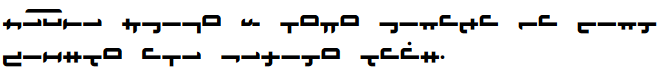
\includegraphics[width=12cm]{desaho.png}
\end{center}

\note{Tekst ten, \emph{ze͞uye chido yi boso hinaja va fint wirklo abe gepito laák}
nie ma większego sensu, ale jest to pangram -- używany jako odpowiednik
polskiego,,pchnąć w tę łódź jeża lub ośm skrzyń fig''.}
\skipline

Ten sam tekst z wykorzystaniem popularnego kroju wzorowanego na piśmie
odręcznym, Na͞epo:

\begin{center}
    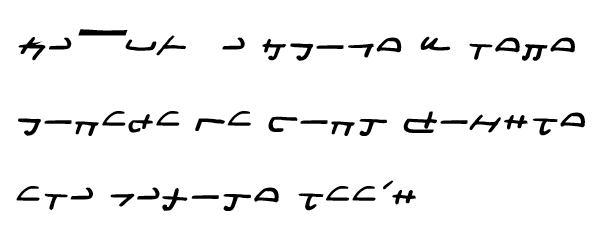
\includegraphics[width=12cm]{naepo.png}
\end{center}

W 2007 roku zaproponowana została transkrypcja androyasańskiego do alfabetu 
łacińskiego (transkrypcja Kadala), poprawiona w~latach 2013 (transkrypcja 
ZSC) i ostatecznie ustalona rok później (transkrypcja Ziri). W~tym słowniku
używana jest tylko i~wyłącznie transkrypcja Ziri.

Język nie jest całkowicie jednorodny -- jako, że włada nim ponad miliard 
użytkowników, pojawiają się w~nim dialekty oraz zachowania i~zasady specyficzne 
dla danej kultury lub regionu. 

Ten słownik skupiać się będzie na literackiej formie języka androyasańskiego,
nazywanej \emph{ardo andro} (wysoki androyasański), pewne uwagi dotyczące
dialektów będą zawarte w~dodatkowych opisach do haseł.

\end{spacing}
% \cleartorecto

% \input{./chapters/writing.tex}
% \cleartorecto

\chapter{Examples}

\glossex{Seja haji.}{seja haji}{Sun shine.PRS}{,,The sun shines.''}
\glossex{Seja vi haji.}{seja vi haji}{Sun IPFV shine.PRS}{,,The sun is shining.''}
\glossex{Ore Seja haji.}{ore seja haji}{now Sun shine.PRS}{,,The sun is shining.''}
\glossex{Seja va hajit.}{seja va haji-t}{sun PFV shine-PST}{,,The sun shone.''}
\glossex{Seja ze haji.}{seja ze haji}{sun FUT shine}{,,The sun will shine.''}
\glossex{Seja vi hajit.}{seja vi haji-t}{sun IPFV shine-PST}{,,The sun has been shining.''}
\glossex{Seja haji rede}{seja haji rede}{sun shine.PRS again}{,,The sun is shining again.''}
\glossex{Seja ze haji zetay}{seja ze haji zetay}{sun FUT shine tomorrow}{,,The sun will shine tomorrow.''}
\glossex{Seja haji siro.}{seja haji siro}{sun shine.PRS bright.ADV}{,,The sun shines brightly.''}
\glossex{Siro Seja haji}{siro seja haji}{bright.ADJ sun shine.PRS}{,,The bright sun shines.''}
\glossex{Seja sormi ore.}{seja sormi ore}{sun sunrise.PRS now}{,,The sun is rising now.''}
\glossex{Sormi ore.}{sormi ore}{sunrise.PRS now}{,,The sun is rising now.''}
\glossex{Recha rujalaros rajit.}{recha rujalar-os raji-t}{all people-PL shout-PST}{,,All the people shouted.''}
\glossex{Recha rajit.}{recha raji-t}{all shout-PST}{,,All the people shouted.''}
\glossex{Noreja rajit.}{noreja raji-t}{some.people shout-PST}{,,Some of the people shouted.''}
\glossex{Vyele rujalaros rajit ka razi.}{vyele rujalar-os raji-t ka razi}{many people-PL shout-PST two times}{,,Many of the people shouted twice.''}
\glossex{Osaker rajit ka razi.}{osaker raji-t ka razi}{many.people shout-PST two times}{,,Many of the people shouted twice.''}
\glossex{Gusto rujalaros rajiri vicho.}{gusto rujalar-os rajiri vicho}{happy people-PL shout.PRS often}{,,Happy people often shout.''}
\glossex{Muchi ka͞ufit ared.}{muchi ka͞ufi-t ared}{kitten jump-PST upward.ADV}{,,The kitten jumped up.''}
\glossex{Muchi ka͞ufit on tasek.}{muchi ka͞ufi-t on tasek}{kitten jump-PST on table}{,,The kitten jumped onto the table.''}
\glossex{Myi vir muchi uneńit.}{myi vir muchi un-eńi-t}{1SG.POSS little cat away-go-PST}{,,My little kitten walked away.''}
\glossex{Aḱame osupi.}{aḱame osupi}{rain fall.PRS}{,,It's raining.''}
\glossex{Aḱame osupit.}{aḱame osupi-t}{rain fall-PST}{,,The rain came down.''}
\glossex{Muchi labi in aḱame.}{muchi labi in aḱame}{cat play.PRS in rain}{,,The kitten is playing in the rain.''}
\glossex{Aḱame aśtot.}{aḱame aśto-t}{rain stop-PST}{,,The rain has stopped.''}
\glossex{Aḱame ze aśtopi naári.}{akame ze aśtopi naári}{rain FUT stop soon}{,,Soon the rain will stop.''}
\glossex{Avi bochada aḱame ze aśtopi naári.}{avi bochada aḱame ze aśtopi naári}{have.PRS hope rain FUT stop soon}{,,I hope the rain stops soon.''}
\glossex{Mosno faji lot volu chet.}{mosno faj-i lo-t volu chet}{wild animal-PL live-PST sometime here}{,,Once wild animals lived here.''}
\glossex{Egla rav́at gepo.}{egl-a rav́a-t gepo}{3SG-F look.around-PST slow.ADV}{,,Slowly she looked around.''}
\glossex{Ti uneńi do!}{ti uneńi do}{2SG go.away IMP}{,,Go away!''}
\glossex{Uneńi do!}{Uneńi do}{go.away IMP}{,,Go away!''}
\glossex{Eni heme!}{eni heme}{go CHR}{,,Let's go!''}
\glossex{Ti vage eni.}{ti vage eni}{2SG HORT go}{,,You should go.''}
\glossex{Vage eni.}{vage eni}{HORT go}{,,You should go.''}
\glossex{Ze esi gusto per eni.}{ze esi gusto per eni}{FUT be happy to.do go}{,,I will be happy to go.''}
\glossex{Egli ze iéni naári.}{egli ze i-éni naári}{3SG.M FUT VEN-go soon}{,,He will arrive soon.''}
\glossex{Chidoyi moroza unj́aret.}{chido-yi moroza un-j́are-t}{child-POSS ball out-roll-PST}{,,The baby's ball has rolled away.''}
\glossex{Ka bovos vi tesuchi.}{ka bov-os vi tesuchi}{two boy-PL IPFV cooperate.PRS}{,,The two boys are working together.''}
\glossex{Ka bovos vi fari tesiko.}{ka bov-os vi fari tesiko}{two boy-PL IPFV work.PRS together.ADV}{,,The two boys are working together.''}
\glossex{Neb́i͞a ze osupi mireisro.}{neb́i͞a ze osupi mireisro}{mist FUT fall probably}{,,This mist will probably clear away.''}
\glossex{Fote͞o flos dolozi in reso.}{fote͞o flo-s dolozi in reso}{lovely.ADJ flower-PL grow.PRS in everywhere}{,,Lovely flowers are growing everywhere.''}
\glossex{Noni vage vibi gepe.}{noni vage vibi gep-e}{1PL HORT eat.PRS slow.ADV-COMP}{,,We should eat more slowly.''}
\glossex{Ti va iént tar chid.}{ti va i-én-t tar chid}{2SG PFV VEN-go-PST too fast.ADV}{,,You have come too soon.''}
\glossex{Ti vipini rizo͞e chiwi.}{ti vipini rizo-e chiwi}{2SG must.PRS.AUX neat-COMP write}{,,You must write more neatly.''}
\glossex{Siniko kebuér varsi rizo onvojibo.}{siniko kebuér varsi rizo onvojibo}{wonderful palace stand.PRS exact.ADV opposite.ADV}{,,Directly opposite stands a wonderful palace.''}
\glossex{Henryi pelir lukat.}{henr-yi pelir luka-t}{henry-POSS dog lose.way-PST}{,,Henry's dog is lost.''}
\glossex{Pelir yi Henri lukat chyi.}{pelir yi henri luka-t chyi}{dog POSS henry lose.way-PST REFL}{,,Henry's dog is lost.''}
\glossex{Myi muche esi ruko.}{myi muche esi ruko}{1SG.POSS cat be.PRS black}{,,My cat is black.''}
\glossex{Myi muche ruko.}{myi muche ruko}{1SG.POSS cat black}{,,My cat is black.''}
\glossex{Loesa yi vir hima esi girefaro.}{loesa yi vir hima esi girefar-o}{doll POSS small girl be.PRS damage-ADJ}{,,The little girl's doll is broken.''}
\glossex{Machagi fahojo inuro.}{machagi fahojo inuro}{sleep.PRS loud.ADV usually.ADV}{,,I usually sleep soundly.''}
\glossex{Chidos jikit mito Jek.}{chid-os jiki-t mito jek}{child-PL run-PST back.ADV jack}{,,The children ran after Jack.''}
\glossex{Epi huhu mibozor labi.}{epi huhu mibozor labi}{can after school play}{,,I can play after school.''}
\glossex{Noni ent o kavala per tamoki.}{noni en-t o kavala per tamoki}{1PL go-PST to village for visit.PRS}{,,We went to the village for a visit.''}
\glossex{Noni iént o aḱumar.}{noni i-én-t o aḱumar}{1PL VEN-go-PST to river}{,,We arrived at the river.''}
\glossex{Va ingek a ti}{va ingek a ti}{PFV wait.PST on 2SG}{,,I have been waiting for you.''}
\glossex{Naberos set ra͞o nafrita.}{naber-os set rao na-frita}{camper-PL sit.PST around camp-fire}{,,The campers sat around the fire.''}
\glossex{Vir hima e il muchi set ne ne͞a mi.}{vir hima e il muchi set nea mi}{small girl and 3SG.POSS kitten sit.PST near.physically 1SG}{,,A little girl with a kitten sat near me.''}
\glossex{Chido ingek a il vapal ner ostro.}{chido ingek a il vapal ner ostro}{child wait.PST on 3SG.POSS father near.physically door}{,,The child waited at the door for her father.''}
\glossex{Kavala yi vyekka hima mant il muchi asweo tay.}{kavala yi vyekka hima man-t il muchi asweo tay}{village POSS old.SUPL girl lose-PST 3SG.POSS kitten previous day}{,,Yesterday the oldest girl in the village lost her kitten.''}
\glossex{Kavala yi vyekka hima yi muchi lukat asweo tay.}{kavala yi vyekka hima yi muchi lukat asweo tay}{village POSS old.SUPL girl POSS kitten lose.way-PST previous day}{,,Yesterday the oldest girl in the village lost her kitten.''}
\glossex{In che kavala ti uńatal?}{in che kavala ti uńatal}{in DEM village 2SG be.born-PST}{,,Were you born in this village?''}
\glossex{Lipe tyi brat leehi?}{lipe tyi brat leehi}{good.ADV 2SG.POSS brother dance}{,,Can your brother dance well?''}
\glossex{Sinit rujaler?}{sini-t rujaler}{leave-PST man}{,,Did the man leave?''}
\glossex{A ti tyi sora iéni?}{a ti tyi sora iéni}{for 2SG 2SG.POSS sister come}{,,Is your sister coming for you?''}
\glossex{Zetay ti epi iéni?}{zetay ti epi iéni}{tomorrow 2SG can.AUX come}{,,Can you come tomorrow?''}
\glossex{Oban mikyimarida ne͞areros va sićherit?}{oban mikyimarida ne͞arer-os va sićheri-t}{for.the.time winter neighbor-PL PFV leave-PST}{,,Have the neighbors gone away for the winter?''}
\glossex{Feban aḱame kahuna kanti?}{feban aḱame kahuna kanti}{during rain bird sing.PRS}{,,Does the robin sing in the rain?''}
\glossex{O kijursa a noni ti ze egi?}{o kijursa a noni ti ze egi}{to concert with 1PL 2SG FUT go}{,,Are you going with us to the concert?''}
\glossex{Volumo churche dalaka ti vayarenit?}{volumo churche dalaka ti vayareni-t}{anywhen.Q through jungle 2SG travel-PST}{,,Have you ever travelled in the jungle?''}
\glossex{Noni fenit aḱumaryi mered churche vyele kilometerdi.}{noni feni-t aḱumar-yi mered churche vyele kilometer-di}{1PL swim-PST river-POSS down through many kilometer-PL}{,,We sailed down the river for several miles.''}
\glossex{Recha saperi on kuanti.}{recha saperi on kuanti}{everybody know.PRS about hunt.PRS}{,,Everybody knows about hunting.''}
\glossex{In sejo zevoyim huhu tayav́al noni sint́epit in abarji.}{in sejo zevoyim huhu tayav́al noni si-nt́epi-t in abar-ji}{in sunny morning after solstice 1PL off-go-PST in mountain-PL}{,,On a Sunny morning after the solstice we started for the mountains.''}
\glossex{Tom chikat dyet chichamayi virfarji.}{tom chika-t dyet chichama-yi virfar-ji}{tom laugh-PST because.of monkey-POSS trick-PL}{,,Tom laughed at the monkey's tricks.''}
\glossex{Vek rujalar one enyasula vajat dyet duloge.}{vek rujalar one enyasula vajat dyet duloge}{old man with walking.stick stand.PST behind fence}{,,An old man with a walking stick stood beside the fence.''}
\glossex{Sukirrayi sehola est kopero chu sif́emo femji.}{sukirra-yi sehola est kopero chu sif́em-o fem-ji}{squirrel-POSS nest be.PST hidden with hang-ADJ branch-PL}{,,The squirrel's nest was hidden by drooping boughs.''}
\glossex{Vir granos ingek tranoko un miker a tepa novekayi seja.}{vir gran-os inge-k tranoko un miker a tepa noveka-yi seja}{tiny seed-PL wait-PST patiently.ADV under snow for warm spring-POSS sun}{,,The little seeds waited patiently under the snow for the warm spring sun.''}
\glossex{Vyele vir hinji one floyi topeka a egyi buutji va leehit ra͞o nafrita.}{vyele vir hin-ji one flo-yi topeka-s a egyi buut-ji va leehi-t ra͞o nafrita}{many little little.girl-PL with flower-POSS wreath-PL physically.on 3PL.POSS head-PL PFV dance-PST around bonfire}{,,Many little girls with wreaths of flowers on their heads danced around the bonfire.''}
\glossex{Iḱopera yi rakel osupet a busama.}{iḱopera yi rakel osup-et a busama}{cover POSS basket fall-PST on floor}{,,The cover of the basket fell to the floor.''}
\glossex{Yelonayi ati bove aśtot ne͞a meńi.}{yelona-yi a-ti bove aśto-t ne͞a meńi}{queue-POSS one-ORD buy stop-PST near entrance}{,,The first boy in the line stopped at the entrance.''}
\glossex{A veray yi varda vek sago hinaja lot in vir wamaga.}{a veray yi varda vek sago hinaja lot-ø in vir wamaga}{on top POSS hill old wise woman live-PST in old hut}{,,On the top of the hill in a little hut lived a wise old woman.''}
\glossex{Feban niyi ewagi na a kavala enidi a filetos vicho.}{feban niyi ewagi na a kavala enidi-t a filet-os vicho}{during 1PL.POSS stay NMLZ on village walk-PST on field-PL often.ADV}{,,During our residence in the country we often walked in the pastures.''}
\glossex{Voli tyi koaleros a͞u espero ze iéni?}{voli tyi koaler-os a͞u espero ze iéni}{when.Q 2SG.POSS guest-PL from city FUT arrive}{,,When will your guests from the city arrive?''}
\glossex{Ner aḱumaryi sina, chyi larima vidi taryo a sormo.}{ner aḱumar-yi sina, chyi larima vidi taryo a sormo}{near.physically river-POSS exit 3.NAN.POSS road turn sharp.ADV on east}{,,Near the mouth of the river, its course turns sharply towards the East.''}
\glossex{Ka ardo abarji bugi menate mereda mede.}{ka ardo abar-ji bugi menate mereda mede}{two high mountain-PL lay fertile valley between.ADV}{,,Between the two lofty mountains lay a fertile valley.''}
\glossex{}{}{}{,,Among the wheat grew tall red poppies.''}
\glossex{}{}{}{,,The strong roots of the oak trees were torn from the ground.''}
\glossex{}{}{}{,,The sun looked down through the branches upon the children at play.''}
\glossex{}{}{}{,,The west wind blew across my face like a friendly caress.''}
\glossex{}{}{}{,,The spool of thread rolled across the floor.''}
\glossex{}{}{}{,,A box of growing plants stood in the Window.''}
\glossex{Mi zosu gusto.}{mi zosu gusto}{1SG very happy}{,,I am very happy.''}
\glossex{}{}{}{,,These oranges are juicy.''}
\glossex{}{}{}{,,Sea water is salty.''}
\glossex{}{}{}{,,The streets are full of people.''}
\glossex{}{}{}{,,Sugar tastes sweet.''}
\glossex{Seiti ifrit votepo.}{seiti ifrit votepo}{feel.PRS fire hot}{,,The fire feels hot.''}
\glossex{Mi seiti ifrit esi votepo.}{mi seiti ifrit esi votepo}{1SG feel.PRS fire be.PRS hot}{,,The fire feels hot.''}
\glossex{Vir hina epit ziralo rori.}{vir hina epi-t ziralo rori}{little girl might-PST lonely think.AUX}{,,The little girl seemed lonely.''}
\glossex{Vir boveyi vapal est suyer volu.}{vir bove-yi vapal es-t suyer volu}{little boy-POSS father be-PST sailor somewhen}{,,The little boy's father had once been a sailor.''}
\glossex{}{}{}{,,I have lost my blanket.''}
\glossex{}{}{}{,,A robin has built his nest in the apple tree.''}
\glossex{}{}{}{,,At noon we ate our lunch by the roadside.''}
\glossex{Jones-epié simoset saler for egi vir bove.}{jones-epié simose-t saler for il vir bove}{jones-HON create-PST knife DAT 3SG.POSS small boy}{,,Mr. Jones made a knife for his little boy.''}
\glossex{Egyi inerji epi rori zosu gusto.}{egyi iner-ji epi.rori zosu gusto}{3PL.POSS voice-PL seem.to.be very happy}{,,Their voices sound very happy.''}
\glossex{Egyi inerji inerai zosu gusto.}{egyi iner-ji inerai zosu gusto}{3PL.POSS voice-PL sound very happy}{,,Their voices sound very happy.''}
\glossex{Atay hetay esi?}{a-tay hetay esi}{first-day today be.PRS}{,,Is today Monday?''}
\glossex{A͞u laák recha ayeri va osupit?}{au laák recha ayer-i va osupi-t}{from tree all leave-PL PFV fall.down-PST}{,,Have all the leaves fallen from the tree?''}
\glossex{Medo voli baán ze esi?}{medo voli baán ze esi}{ready when time FUT be}{,,Will you be ready on time?''}
\glossex{Missani fo mi ti ze siyurchi?}{missani fo mi ti ze siyurchi}{message DAT 1SG 2SG FUT send}{,,Will you send this message for me?''}
\glossex{Vi ingeki a mi?}{vi ingeki a mi}{IPFV wait for 1SG}{,,Are you waiting for me?''}
\glossex{}{}{}{,,Is this the first kitten of the litter?''}
\glossex{Tur gruwe fo ti je kutos esi?}{tur gruwe fo yi je kutos esi}{too big DAT 2SG DEM shoe.PL be.PRS}{,,Are these shoes too big for you?''}
\glossex{Ali wa͞ime aḱumar esi?}{ali wa͞ime aḱumar esi}{how.much.Q wide river be.PRS}{,,How wide is the River?''}
\glossex{Vage kaéti.}{vage kaéti}{HORT listen}{,,Listen.''}
\glossex{Kaéti do.}{kaéti do}{listen IMP}{,,Listen.''}
\glossex{Seysi chet ne͞a myi do.}{seysi chet ne͞a myi do}{sit here near 1SG.ACC IMP}{,,Sit here by me.''}
\glossex{}{}{}{,,Keep this secret until tomorrow.''}
\glossex{Tesiko noni eni heme.}{tesiko noni eni heme}{together 1PL go CHR}{,,Come with us.''}
\glossex{}{}{}{,,Bring your friends with you.''}
\glossex{}{}{}{,,Be careful.''}
\glossex{}{}{}{,,Have some tea.''}
\glossex{Pip e il pelir est lipe alyes.}{Pip e il pelir est lipe alye-s}{Pip and 3SG.POSS dog be.PST good friend-PL}{,,Pip and his dog were great friends.''}
\glossex{Jon e Elizabet esi brat e sora}{Jon e Elizabet esi brat e sora}{John and Elizabeth be.PRS brother and sister}{,,John and Elizabeth are brother and sister.''}
\glossex{Ti e mi ze eni tesiko.}{ti e mi ze eni tesiko}{2SG and 1SG FUT go together.ADV}{,,You and I will go together.''}
\glossex{Ego͞i id́ak recha ostros e dakos.}{ego͞i id́ak recha ostro-s e dako-s}{3PL open.PST every door-PL and window-PL}{,,They opened all the doors and windows.''}
\glossex{Egi esi vir, abe valor.}{egi esi vir abe valor}{3SG be small but strong}{,,He is small, but strong.''}
\glossex{}{}{}{,,Is this tree an oak or a maple?''}
\glossex{Arso zor stobo ari esi?}{arso zor stobo ari esi}{azure exclusive.or gray sky be.PRS}{,,Does the sky look blue or gray?''}
\glossex{Vage iéni a vapal yen natali͞a.}{vage iéni a vapal yen natali͞a}{HORT come together.with father or mother}{,,Come with your father or mother.''}
\glossex{Mi ge payto esi, abe zosu gusto.}{mi ge payt-o esi abe zosu gusto}{1SG PASS tire-ADJ but very happy}{,,I am tired, but very happy.''}
\glossex{}{}{}{,,He played a tune on his wonderful flute.''}
\glossex{}{}{}{,,Toward the end of August the days grow much shorter.''}
\glossex{}{}{}{,,A company of soldiers marched over the hill and across the meadow.''}
\glossex{Ati taúnin yi yeitto zosu intrise.}{a-ti taúnin yi yeitto zosu intrise}{one-ORD part POSS story very interesting}{,,The first part of the story is very interesting.''}
\glossex{}{}{}{,,The crow dropped some pebbles into the pitcher and raised the water to the brim.''}
\glossex{}{}{}{,,The baby clapped her hands and laughed in glee.''}
\glossex{Fiji aśtopi e esi yubo do.}{fiji astopi e esi yubo do}{game.PRS stop.PRS and be.PRS quiet.ADV IMP}{,,Stop your game and be quiet.''}
\glossex{}{}{}{,,The sound of the drums grew louder and louder.''}
\glossex{Samos zor mikyimarida ti anvi?}{samos ji mikyimarida ti anvi}{summer or winter 2SG prefer}{,,Do you like summer or winter better?''}
\glossex{}{}{}{,,That boy will have a wonderful trip.''}
\glossex{}{}{}{,,They popped corn, and then sat around the fire and ate it.''}
\glossex{}{}{}{,,They won the first two games, but lost the last one.''}
\glossex{}{}{}{,,Take this note, carry it to your mother; and wait for an answer.''}
\glossex{}{}{}{,,I awoke early, dressed hastily, and went down to breakfast.''}
\glossex{Aha! Va kanit ti!}{aha va kani-t ti}{aha PFV catch-PST 2SG}{,,Aha! I have caught you!''}
\glossex{}{}{}{,,This string is too short!''}
\glossex{}{}{}{,,Oh, dear! the wind has blown my hat away!''}
\glossex{}{}{}{,,Alas! that news is sad indeed!''}
\glossex{}{}{}{,,Whew! that cold wind freezes my nose!''}
\glossex{}{}{}{,,Are you warm enough now?''}
\glossex{}{}{}{,,They heard the warning too late.''}
\glossex{}{}{}{,,We are a brave people, and love our country.''}
\glossex{Recha chidos aygo Meri iént.}{recha chid-os aygo Meri iént}{all.of child-PL apart.from Mary come.PST}{,,All the children came except Mary.''}
\glossex{}{}{}{,,Jack seized a handful of pebbles and threw them into the lake.''}
\glossex{}{}{}{,,This cottage stood on a low hill, at some distance from the village.''}
\glossex{}{}{}{,,On a fine summer evening, the two old people were sitting outside the door of their cottage.''}
\glossex{}{}{}{,,Our bird's name is Jacko.''}
\glossex{}{}{}{,,The river knows the way to the sea.''}
\glossex{}{}{}{,,The boat sails away, like a bird on the wing.''}
\glossex{}{}{}{,,They looked cautiously about, but saw nothing.''}
\glossex{}{}{}{,,The little house had three rooms, a sitting room, a bedroom, and a tiny kitchen.''}
\glossex{}{}{}{,,We visited my uncle's village, the largest village in the world.''}
\glossex{}{}{}{,,We learn something new each day.''}
\glossex{}{}{}{,,The market begins five minutes earlier this week.''}
\glossex{}{}{}{,,Did you find the distance too great?''}
\glossex{}{}{}{,,Hurry, children.''}
\glossex{}{}{}{,,Madam, I will obey your command.''}
\glossex{}{}{}{,,Here under this tree they gave their guests a splendid feast.''}
\glossex{}{}{}{,,In winter I get up at night, and dress by yellow candlelight.''}
\glossex{}{}{}{,,Tell the last part of that story again.''}
\glossex{}{}{}{,,Be quick or you will be too late.''}
\glossex{}{}{}{,,Will you go with us or wait here?''}
\glossex{}{}{}{,,She was always, shabby, often ragged, and on cold days very uncomfortable.''}
\glossex{}{}{}{,,Think first and then act.''}
\glossex{}{}{}{,,I stood, a little mite of a girl, upon a chair by the window, and watched the falling snowflakes.''}
\glossex{}{}{}{,,Show the guests these shells, my son, and tell them their strange history.''}
\glossex{}{}{}{,,Be satisfied with nothing but your best.''}
\glossex{}{}{}{,,We consider them our faithful friends.''}
\glossex{}{}{}{,,We will make this place our home.''}
\glossex{}{}{}{,,The squirrels make their nests warm and snug with soft moss and leaves.''}
\glossex{}{}{}{,,The little girl made the doll's dress herself.''}
\glossex{}{}{}{,,I hurt myself.''}
\glossex{}{}{}{,,She was talking to herself.''}
\glossex{}{}{}{,,He proved himself trustworthy.''}
\glossex{}{}{}{,,We could see ourselves in the water.''}
\glossex{}{}{}{,,Do it yourself.''}
\glossex{}{}{}{,,I feel ashamed of myself.''}
\glossex{}{}{}{,,Sit here by yourself.''}
\glossex{}{}{}{,,The dress of the little princess was embroidered with roses, the national flower of the Country.''}
\glossex{}{}{}{,,They wore red caps, the symbol of liberty.''}
\glossex{}{}{}{,,With him as our protector, we fear no danger.''}
\glossex{}{}{}{,,All her finery, lace, ribbons, and feathers, was packed away in a trunk.''}
\glossex{}{}{}{,,Light he thought her, like a feather.''}
\glossex{}{}{}{,,Every spring and fall our cousins pay us a long visit.''}
\glossex{}{}{}{,,In our climate the grass remains green all winter.''}
\glossex{}{}{}{,,The boy who brought the book has gone.''}
\glossex{}{}{}{,,These are the flowers that you ordered.''}
\glossex{}{}{}{,,I have lost the book that you gave me.''}
\glossex{}{}{}{,,The fisherman who owned the boat now demanded payment.''}
\glossex{}{}{}{,,Come when you are called.''}
\glossex{}{}{}{,,I shall stay at home if it rains.''}
\glossex{}{}{}{,,When he saw me, he stopped.''}
\glossex{}{}{}{,,Do not laugh at me because I seem so absent minded.''}
\glossex{}{}{}{,,I shall lend you the books that you need.''}
\glossex{}{}{}{,,Come early next Monday if you can.''}
\glossex{}{}{}{,,If you come early, wait in the hall.''}
\glossex{}{}{}{,,I had a younger brother whose name was Antonio.''}
\glossex{}{}{}{,,Gnomes are little men who live under the ground.''}
\glossex{}{}{}{,,He is loved by everybody, because he has a gentle disposition.''}
\glossex{}{}{}{,,Hold the horse while I run and get my cap.''}
\glossex{}{}{}{,,I have found the ring I lost.''}
\glossex{}{}{}{,,Play and I will sing.''}
\glossex{}{}{}{,,That is the funniest story I ever heard.''}
\glossex{}{}{}{,,She is taller than her brother.''}
\glossex{}{}{}{,,They are no wiser than we.''}
\glossex{}{}{}{,,Light travels faster than sound.''}
\glossex{}{}{}{,,We have more time than they.''}
\glossex{}{}{}{,,She has more friends than enemies.''}
\glossex{}{}{}{,,He was very poor, and with his wife and five children lived in a little low cabin of logs and stones.''}
\glossex{}{}{}{,,When the wind blew, the traveler wrapped his mantle more closely around him.''}
\glossex{}{}{}{,,I am sure that we can go.''}
\glossex{}{}{}{,,We went back to the place where we saw the roses.''}
\glossex{}{}{}{,,"This tree is fifty feet high," said the gardener.''}
\glossex{}{}{}{,,I think that this train leaves five minutes earlier today.''}
\glossex{}{}{}{,,My opinion is that the governor will grant him a pardon.''}
\glossex{}{}{}{,,Why he has left the city is a mystery.''}
\glossex{}{}{}{,,The house stands where three roads meet.''}
\glossex{}{}{}{,,He has far more money than brains.''}
\glossex{}{}{}{,,Evidently that gate is never opened, for the long grass and the great hemlocks grow close against it.''}
\glossex{}{}{}{,,I met a little cottage girl; she was eight years old, she said.''}
\glossex{Noni ge siyurchet per karli chu e͞iger e zaálta.}{noni ge siyurche-t per karli chu e͞iger e zaálta}{1PL PASS send-PST for die.PRS ACC emperor and nation}{,,We were sent to die for the emperor and nation.''}
\glossex{Abejar voli koboviros karli, egyi natalji inrit.}{abejar voli kobovir-os kar-et, egyi natalji inri-t}{however when soldier-PL die-PST 3PL.POSS mother-PL call-PST}{,,But when the soldiers were dying, called out to their mothers.''}
\glossex{Moĺi kaét sotak chu egi e͞iger e zaálta vi inrit.}{moĺi kaét sotak chu egi e͞iger e zaálta vi inri-t}{never hear.PST someone ACC 3SG emperor and nation IPFV call-PST}{,,I never heard anyone calling the emperor and the nation.''}
\glossex{Vage loti lipe lot.}{vage loti lipe lot}{HORT live.PRS good life}{,,Live a good life.''}
\glossex{Miam ora͞i feśidari e licho esi vimi ze siti no ali ti horo est.}{miam ora͞i feśidari e licho esi vimi ze siti no ali ti horo est}{if god.PL exist.PRS and just be.PRS then FUT interest NEG how.many 2SG devout be.PST}{,,If there are gods and they are just, then they will not care how devout you have been.''}
\glossex{Miam ora͞i feśidari, abe nolicho, vimi ti egyi ori vage teviti no.}{miam ora͞i feśidari abe no-licho vimi ti egyi ori vage teviti no}{if god.PL exist but NEG-just then 2SG 3PL.ACC worship HORT want NEG}{,,If there are gods, but unjust, then you should not want to worship them.''}
\glossex{Miam ora͞i feśidari no, vimi ti uneńit, abejar vi lot arujaro lot chu ze vi feśidari in saypes yi tyi koólerji.}{miam ora͞i feśidari no vimi ti ze uneńi abejar vi lot arujaro lot chu ze vi feśidari in saype-s yi tyi koóler-ji}{if god.PL exist NEG then 2SG FUT leave however IPFV live.PST noble.ADV ACC IPFV exist in memory-PL POSS 2SG.POSS loved.one-PL}{,,If there are no gods, then you will be gone, but will have lived a noble life that will live on in the memories of your loved ones.''}
\glossex{Baljejet joifina flos no.}{baljeje-t joifina flo-s no}{receive-PST kick-NMLZ flower-PL instead.of}{I got a kick instead of flowers.}
\glossex{Akaro arios sormi an kavala ge dozit da ichera.}{akar-o arios sormi an kavala ge dozi-t da ichera}{red-ADJ Moon rise.PRS over village PASS make.dirty-PST INS blood}{,,The red Moon is rising over a village smeared with blood.''}
\glossex{Tyi gont ze stani no o voli tay in chu recha vireji uf́riti ze iéni.}{tyi gont ze stani no o=voli tay in chu recha vire-ji ze uf́riti ze i-éni}{2SG.POSS soul FUT rest.PRS NEG until day LOC GEN all star-PL FUT burn.out FUT VEN-come}{,,Your soul will not rest until comes the day in which all stars will burn out.''}
\glossex{Egla esi merlio fo mi.}{egl-a esi merlio fo mi}{3SG.F be.PRS appealing.ADJ DAT 1SG}{,,She is pretty in my opinion.'' \\ ,,She is appealing to me'' \\ ,,I like her.''}
\glossex{Egla merlio fo mi.}{egl-a merlio fo mi}{3SG.F appealing.ADJ DAT 1SG}{,,She is pretty in my opinion.'' \\ ,,She is appealing to me'' \\ ,,I like her.''}
\glossex{Egla merlio mi.}{egl-a merlio mi}{3SG.F appealing.ADJ 1SG}{,,She is pretty in my opinion.'' \\ ,,She is appealing to me'' \\ ,,I like her.''}
\glossex{Egla merlio.}{egl-a merlio}{3SG.F appealing.ADJ}{,,She is pretty in my opinion.'' \\ ,,She is appealing to me'' \\ ,,I like her.''}
\glossex{Mi ya egla merlio.}{mi ya egl-a merlio}{1SG TOP 3SG.F appealing.ADJ}{,,As for my opinion, she is pretty.'' \\ ,,She is pretty in my opinion.''}

\cleartorecto

%% BACK MATTER %%%%%%%%%%%%%%%%%%%%%%%%%%%%%%%%%%%%%%%%%%%%%%%%%%%%%%%%%%%%%%%%

\backmatter

\begingroup\multicolsep=0pt
%\printindex
\endgroup

\end{document}